% -----------------------------------------------------------------------------
%                                     HEADER                                    
% -----------------------------------------------------------------------------
\documentclass[a4paper, 10pt]{article}
\usepackage{jheppub}
\usepackage[T1]{fontenc}
\usepackage{colortbl,xcolor,float}
\definecolor{orange}{rgb}{1,0.5,0}
% -----------------------------------------------------------------------------
%                                   COVER PAGE                                  
% -----------------------------------------------------------------------------
\title{{
\includegraphics[scale=.4]{logo.eps}}\ The LaTeX report}

\author{Generated by elijahsheridan on 04 September 2020, 02:57:17}

\abstract{
  This report has been generated automatically
  by {\sc MadAnalysis} 5.\\$~$\\ 
  Please cite:\\ 
  \begin{quote}
    \textbf{E.~Conte, B.~Fuks and G.~Serret},\\ 
    \textit{MadAnalysis 5, A User-Friendly
    Framework for Collider Phenomenology},\\ 
    Comput. Phys. Commun. {\bf 184} (2013) 222-256,\\
    arXiv:1206.1599 [hep-ph].\\ 
  \end{quote}
  To contact us:\\ 
  \begin{quote}
    \textbf{http://madanalysis.irmp.ucl.ac.be}\\
    \textbf{ma5team@iphc.cnrs.fr}\\
  \end{quote}
}

% -----------------------------------------------------------------------------
%                                 BEGIN DOCUMENT                                
% -----------------------------------------------------------------------------
\begin{document}
\maketitle
\flushbottom

% -----------------------------------------------------------------------------
%                                 SECTION Setup                                 
% -----------------------------------------------------------------------------
\newpage
\section{ Setup}

\subsection{ Command history}

\texttt{ma5>\# set directory where running "./\-bin/\-ma5"; set lumi; define the signal significance\\
}
\texttt{ }\texttt{ }\texttt{ma5>set main.currentdir = /\-Users/\-elijahsheridan/\-MG5\_aMC\_v2\_6\_5/\-axion\_pheno/\-madgraph\_data \# need to change this directory path --> exit and type "pwd" to get the path\\
}
\texttt{ }\texttt{ }\texttt{ma5>set main.lumi = 40\\
}
\texttt{ }\texttt{ }\texttt{ma5>set main.fom.formula = 5\\
}
\texttt{ }\texttt{ }\texttt{ma5>set main.fom.x = 0.25\\
}
\texttt{ }\texttt{ }\texttt{ma5>\# import samples --> change the path to the LHE file\\
}
\texttt{ }\texttt{ }\texttt{ma5>import /\-Users/\-elijahsheridan/\-MG5\_aMC\_v2\_6\_5/\-axion\_pheno/\-madgraph\_data/\-axion\_signal/\-signal\_120mjj\_2deta\_100MeVma\_2TeVL/\-ma100MeV\_L2TeV\_deta2.lhe as signal\\
}
\texttt{ }\texttt{ }\texttt{ma5>import /\-Users/\-elijahsheridan/\-MG5\_aMC\_v2\_6\_5/\-axion\_pheno/\-madgraph\_data/\-diphoton\_double\_isr\_background\_data/\-merged\_lhe/\-diphoton\_double\_isr\_background\_ht\_0\_100\_merged.lhe.gz as bg\_dip\_0\_100\\
}
\texttt{ }\texttt{ }\texttt{ma5>import /\-Users/\-elijahsheridan/\-MG5\_aMC\_v2\_6\_5/\-axion\_pheno/\-madgraph\_data/\-diphoton\_double\_isr\_background\_data/\-merged\_lhe/\-diphoton\_double\_isr\_background\_ht\_100\_200\_merged.lhe.gz as bg\_dip\_100\_200\\
}
\texttt{ }\texttt{ }\texttt{ma5>import /\-Users/\-elijahsheridan/\-MG5\_aMC\_v2\_6\_5/\-axion\_pheno/\-madgraph\_data/\-diphoton\_double\_isr\_background\_data/\-merged\_lhe/\-diphoton\_double\_isr\_background\_ht\_200\_400\_merged.lhe.gz as bg\_dip\_200\_400\\
}
\texttt{ }\texttt{ }\texttt{ma5>import /\-Users/\-elijahsheridan/\-MG5\_aMC\_v2\_6\_5/\-axion\_pheno/\-madgraph\_data/\-diphoton\_double\_isr\_background\_data/\-merged\_lhe/\-diphoton\_double\_isr\_background\_ht\_400\_600\_merged.lhe.gz as bg\_dip\_400\_600\\
}
\texttt{ }\texttt{ }\texttt{ma5>import /\-Users/\-elijahsheridan/\-MG5\_aMC\_v2\_6\_5/\-axion\_pheno/\-madgraph\_data/\-diphoton\_double\_isr\_background\_data/\-merged\_lhe/\-diphoton\_double\_isr\_background\_ht\_600\_800\_merged.lhe.gz as bg\_dip\_600\_800\\
}
\texttt{ }\texttt{ }\texttt{ma5>import /\-Users/\-elijahsheridan/\-MG5\_aMC\_v2\_6\_5/\-axion\_pheno/\-madgraph\_data/\-diphoton\_double\_isr\_background\_data/\-merged\_lhe/\-diphoton\_double\_isr\_background\_ht\_800\_1200\_merged.lhe.gz as bg\_dip\_800\_1200\\
}
\texttt{ }\texttt{ }\texttt{ma5>import /\-Users/\-elijahsheridan/\-MG5\_aMC\_v2\_6\_5/\-axion\_pheno/\-madgraph\_data/\-diphoton\_double\_isr\_background\_data/\-merged\_lhe/\-diphoton\_double\_isr\_background\_ht\_1200\_1600\_merged.lhe.gz as bg\_dip\_1200\_1600\\
}
\texttt{ }\texttt{ }\texttt{ma5>import /\-Users/\-elijahsheridan/\-MG5\_aMC\_v2\_6\_5/\-axion\_pheno/\-madgraph\_data/\-diphoton\_double\_isr\_background\_data/\-merged\_lhe/\-diphoton\_double\_isr\_background\_ht\_1600\_inf\_merged.lhe.gz as bg\_dip\_1600\_inf\\
}
\texttt{ }\texttt{ }\texttt{ma5>import /\-Users/\-elijahsheridan/\-MG5\_aMC\_v2\_6\_5/\-axion\_pheno/\-madgraph\_data/\-vbf\_diphoton\_background\_data/\-merged\_lhe/\-vbf\_diphoton\_background\_ht\_0\_100\_merged.lhe.gz as bg\_vbf\_0\_100\\
}
\texttt{ }\texttt{ }\texttt{ma5>import /\-Users/\-elijahsheridan/\-MG5\_aMC\_v2\_6\_5/\-axion\_pheno/\-madgraph\_data/\-vbf\_diphoton\_background\_data/\-merged\_lhe/\-vbf\_diphoton\_background\_ht\_100\_200\_merged.lhe.gz as bg\_vbf\_100\_200\\
}
\texttt{ }\texttt{ }\texttt{ma5>import /\-Users/\-elijahsheridan/\-MG5\_aMC\_v2\_6\_5/\-axion\_pheno/\-madgraph\_data/\-vbf\_diphoton\_background\_data/\-merged\_lhe/\-vbf\_diphoton\_background\_ht\_200\_400\_merged.lhe.gz as bg\_vbf\_200\_400\\
}
\texttt{ }\texttt{ }\texttt{ma5>import /\-Users/\-elijahsheridan/\-MG5\_aMC\_v2\_6\_5/\-axion\_pheno/\-madgraph\_data/\-vbf\_diphoton\_background\_data/\-merged\_lhe/\-vbf\_diphoton\_background\_ht\_400\_600\_merged.lhe.gz as bg\_vbf\_400\_600\\
}
\texttt{ }\texttt{ }\texttt{ma5>import /\-Users/\-elijahsheridan/\-MG5\_aMC\_v2\_6\_5/\-axion\_pheno/\-madgraph\_data/\-vbf\_diphoton\_background\_data/\-merged\_lhe/\-vbf\_diphoton\_background\_ht\_600\_800\_merged.lhe.gz as bg\_vbf\_600\_800\\
}
\texttt{ }\texttt{ }\texttt{ma5>import /\-Users/\-elijahsheridan/\-MG5\_aMC\_v2\_6\_5/\-axion\_pheno/\-madgraph\_data/\-vbf\_diphoton\_background\_data/\-merged\_lhe/\-vbf\_diphoton\_background\_ht\_800\_1200\_merged.lhe.gz as bg\_vbf\_800\_1200\\
}
\texttt{ }\texttt{ }\texttt{ma5>import /\-Users/\-elijahsheridan/\-MG5\_aMC\_v2\_6\_5/\-axion\_pheno/\-madgraph\_data/\-vbf\_diphoton\_background\_data/\-merged\_lhe/\-vbf\_diphoton\_background\_ht\_1200\_1600\_merged.lhe.gz as bg\_vbf\_1200\_1600\\
}
\texttt{ }\texttt{ }\texttt{ma5>import /\-Users/\-elijahsheridan/\-MG5\_aMC\_v2\_6\_5/\-axion\_pheno/\-madgraph\_data/\-vbf\_diphoton\_background\_data/\-merged\_lhe/\-vbf\_diphoton\_background\_ht\_1600\_inf\_merged.lhe.gz as bg\_vbf\_1600\_inf\\
}
\texttt{ }\texttt{ }\texttt{ma5>\# define bg and signal samples\\
}
\texttt{ }\texttt{ }\texttt{ma5>set signal.type = signal\\
}
\texttt{ }\texttt{ }\texttt{ma5>set bg\_vbf\_0\_100.type = background\\
}
\texttt{ }\texttt{ }\texttt{ma5>set bg\_vbf\_100\_200.type = background\\
}
\texttt{ }\texttt{ }\texttt{ma5>set bg\_vbf\_200\_400.type  = background\\
}
\texttt{ }\texttt{ }\texttt{ma5>set bg\_vbf\_400\_600.type  = background\\
}
\texttt{ }\texttt{ }\texttt{ma5>set bg\_vbf\_600\_800.type  = background\\
}
\texttt{ }\texttt{ }\texttt{ma5>set bg\_vbf\_800\_1200.type  = background\\
}
\texttt{ }\texttt{ }\texttt{ma5>set bg\_vbf\_1200\_1600.type  = background\\
}
\texttt{ }\texttt{ }\texttt{ma5>set bg\_vbf\_1600\_inf.type = background\\
}
\texttt{ }\texttt{ }\texttt{ma5>set bg\_dip\_0\_100.type = background\\
}
\texttt{ }\texttt{ }\texttt{ma5>set bg\_dip\_100\_200.type = background\\
}
\texttt{ }\texttt{ }\texttt{ma5>set bg\_dip\_200\_400.type = background\\
}
\texttt{ }\texttt{ }\texttt{ma5>set bg\_dip\_400\_600.type = background\\
}
\texttt{ }\texttt{ }\texttt{ma5>set bg\_dip\_600\_800.type = background\\
}
\texttt{ }\texttt{ }\texttt{ma5>set bg\_dip\_800\_1200.type = background\\
}
\texttt{ }\texttt{ }\texttt{ma5>set bg\_dip\_1200\_1600.type = background\\
}
\texttt{ }\texttt{ }\texttt{ma5>set bg\_dip\_1600\_inf.type = background\\
}
\texttt{ }\texttt{ }\texttt{ma5>\# a jet can be from a light quark or b quark\\
}
\texttt{ }\texttt{ }\texttt{ma5>define jets = j\\
}
\texttt{ }\texttt{ }\texttt{ma5>define e = e+ e-\\
}
\texttt{ }\texttt{ }\texttt{ma5>define mu = mu+ mu-\\
}
\texttt{ }\texttt{ }\texttt{ma5>define ta = ta+ ta-\\
}
\texttt{ }\texttt{ }\texttt{ma5>define lept = e mu ta\\
}
\texttt{ }\texttt{ }\texttt{ma5>define ax = 9000005\\
}
\texttt{ }\texttt{ }\texttt{ma5>\# cuts\\
}
\texttt{ }\texttt{ }\texttt{ma5>select ((sdETA(jets[1] jets[2]) > 2 or sdETA(jets[1] jets[2]) < -2) and M(jets[1] jets[2]) > 750) and (PT(a[1]) > 300 and M(a[1] a[2]) > 500)\\
}
\texttt{ }\texttt{ }\texttt{ma5>\# define which plots to make\\
}
\texttt{ }\texttt{ }\texttt{ma5>plot PT(jets[1])\\
}
\texttt{ }\texttt{ }\texttt{ma5>plot ETA(jets[1])\\
}
\texttt{ }\texttt{ }\texttt{ma5>plot PHI(jets[1])\\
}
\texttt{ }\texttt{ }\texttt{ma5>plot PT(jets[2])\\
}
\texttt{ }\texttt{ }\texttt{ma5>plot ETA(jets[2])\\
}
\texttt{ }\texttt{ }\texttt{ma5>plot PHI(jets[2])\\
}
\texttt{ }\texttt{ }\texttt{ma5>plot DELTAR(jets[1], jets[2])\\
}
\texttt{ }\texttt{ }\texttt{ma5>plot M(jets[1] jets[2])\\
}
\texttt{ }\texttt{ }\texttt{ma5>plot sdETA(jets[1] jets[2])\\
}
\texttt{ }\texttt{ }\texttt{ma5>plot M(a[1] a[2])\\
}
\texttt{ }\texttt{ }\texttt{ma5>plot PT(a[1])\\
}
\texttt{ }\texttt{ }\texttt{ma5>plot PT(a[2])\\
}
\texttt{ }\texttt{ }\texttt{ma5>plot THT\\
}
\texttt{ }\texttt{ }\texttt{ma5>plot MET\\
}
\texttt{ }\texttt{ }\texttt{ma5>plot TET\\
}
\texttt{ }\texttt{ }\texttt{ma5>\#set the plot/\-graph parameters\\
}
\texttt{ }\texttt{ }\texttt{ma5>set selection[2].xmin = 0\\
}
\texttt{ }\texttt{ }\texttt{ma5>set selection[2].xmax = 2000\\
}
\texttt{ }\texttt{ }\texttt{ma5>set selection[2].nbins = 200\\
}
\texttt{ }\texttt{ }\texttt{ma5>set selection[2].rank = PTordering\\
}
\texttt{ }\texttt{ }\texttt{ma5>set selection[2].titleX = "p\_\{T\}[j\_\{1\}] (GeV)"\\
}
\texttt{ }\texttt{ }\texttt{ma5>set selection[3].xmin = -8\\
}
\texttt{ }\texttt{ }\texttt{ma5>set selection[3].xmax = 8\\
}
\texttt{ }\texttt{ }\texttt{ma5>set selection[3].nbins = 160\\
}
\texttt{ }\texttt{ }\texttt{ma5>set selection[3].rank = PTordering\\
}
\texttt{ }\texttt{ }\texttt{ma5>set selection[3].titleX = "\#eta[j\_\{1\}]"\\
}
\texttt{ }\texttt{ }\texttt{ma5>set selection[4].xmin = -3.2\\
}
\texttt{ }\texttt{ }\texttt{ma5>set selection[4].xmax = 3.2\\
}
\texttt{ }\texttt{ }\texttt{ma5>set selection[4].nbins = 64\\
}
\texttt{ }\texttt{ }\texttt{ma5>set selection[4].rank = PTordering\\
}
\texttt{ }\texttt{ }\texttt{ma5>set selection[4].titleX = "\#phi[j\_\{1\}]"\\
}
\texttt{ }\texttt{ }\texttt{ma5>set selection[5].xmin = 0\\
}
\texttt{ }\texttt{ }\texttt{ma5>set selection[5].xmax = 1000\\
}
\texttt{ }\texttt{ }\texttt{ma5>set selection[5].nbins = 100\\
}
\texttt{ }\texttt{ }\texttt{ma5>set selection[5].rank = PTordering\\
}
\texttt{ }\texttt{ }\texttt{ma5>set selection[5].titleX = "p\_\{T\}[j\_\{2\}] (GeV)"\\
}
\texttt{ }\texttt{ }\texttt{ma5>set selection[6].xmin = -8\\
}
\texttt{ }\texttt{ }\texttt{ma5>set selection[6].xmax = 8\\
}
\texttt{ }\texttt{ }\texttt{ma5>set selection[6].nbins = 160\\
}
\texttt{ }\texttt{ }\texttt{ma5>set selection[6].rank = PTordering\\
}
\texttt{ }\texttt{ }\texttt{ma5>set selection[6].titleX = "\#eta[j\_\{2\}]"\\
}
\texttt{ }\texttt{ }\texttt{ma5>set selection[7].xmin = -3.2\\
}
\texttt{ }\texttt{ }\texttt{ma5>set selection[7].xmax = 3.2\\
}
\texttt{ }\texttt{ }\texttt{ma5>set selection[7].nbins = 64\\
}
\texttt{ }\texttt{ }\texttt{ma5>set selection[7].rank = PTordering\\
}
\texttt{ }\texttt{ }\texttt{ma5>set selection[7].titleX = "\#phi[j\_\{2\}]"\\
}
\texttt{ }\texttt{ }\texttt{ma5>set selection[8].xmin = 0\\
}
\texttt{ }\texttt{ }\texttt{ma5>set selection[8].xmax = 15\\
}
\texttt{ }\texttt{ }\texttt{ma5>set selection[8].nbins = 75\\
}
\texttt{ }\texttt{ }\texttt{ma5>set selection[8].rank = PTordering\\
}
\texttt{ }\texttt{ }\texttt{ma5>set selection[8].titleX = "\#DeltaR[j\_\{1\},j\_\{2\}]"\\
}
\texttt{ }\texttt{ }\texttt{ma5>set selection[9].xmin = 750\\
}
\texttt{ }\texttt{ }\texttt{ma5>set selection[9].xmax = 8000\\
}
\texttt{ }\texttt{ }\texttt{ma5>set selection[9].nbins = 160\\
}
\texttt{ }\texttt{ }\texttt{ma5>set selection[9].rank = PTordering\\
}
\texttt{ }\texttt{ }\texttt{ma5>set selection[9].titleX = "M[j\_\{1\},j\_\{2\}] (GeV)"\\
}
\texttt{ }\texttt{ }\texttt{ma5>set selection[10].xmin = 2\\
}
\texttt{ }\texttt{ }\texttt{ma5>set selection[10].xmax = 15\\
}
\texttt{ }\texttt{ }\texttt{ma5>set selection[10].titleX = "\#Delta\#eta(j\_\{1\},j\_\{2\})"\\
}
\texttt{ }\texttt{ }\texttt{ma5>set selection[11].xmin = 500\\
}
\texttt{ }\texttt{ }\texttt{ma5>set selection[11].xmax = 4000\\
}
\texttt{ }\texttt{ }\texttt{ma5>set selection[11].nbins = 400\\
}
\texttt{ }\texttt{ }\texttt{ma5>set selection[11].rank = PTordering\\
}
\texttt{ }\texttt{ }\texttt{ma5>set selection[11].titleX = "M[a\_\{1\},a\_\{2\}] (GeV)"\\
}
\texttt{ }\texttt{ }\texttt{ma5>set selection[12].xmin = 300\\
}
\texttt{ }\texttt{ }\texttt{ma5>set selection[12].xmax = 2000\\
}
\texttt{ }\texttt{ }\texttt{ma5>set selection[12].nbins = 80\\
}
\texttt{ }\texttt{ }\texttt{ma5>set selection[12].rank = PTordering\\
}
\texttt{ }\texttt{ }\texttt{ma5>set selection[12].titleX = "p\_\{T\}[a\_\{1\}]"\\
}
\texttt{ }\texttt{ }\texttt{ma5>set selection[13].xmin = 0\\
}
\texttt{ }\texttt{ }\texttt{ma5>set selection[13].xmax = 2000\\
}
\texttt{ }\texttt{ }\texttt{ma5>set selection[13].nbins = 400\\
}
\texttt{ }\texttt{ }\texttt{ma5>set selection[13].rank = PTordering\\
}
\texttt{ }\texttt{ }\texttt{ma5>set selection[13].titleX = "p\_\{T\}[a\_\{2\}] (GeV)"\\
}
\texttt{ }\texttt{ }\texttt{ma5>set selection[14].xmin = 0\\
}
\texttt{ }\texttt{ }\texttt{ma5>set selection[14].xmax = 4000\\
}
\texttt{ }\texttt{ }\texttt{ma5>set selection[14].nbins = 80\\
}
\texttt{ }\texttt{ }\texttt{ma5>set selection[14].rank = PTordering\\
}
\texttt{ }\texttt{ }\texttt{ma5>set selection[14].titleX = "THT"\\
}
\texttt{ }\texttt{ }\texttt{ma5>set selection[15].xmin = 0\\
}
\texttt{ }\texttt{ }\texttt{ma5>set selection[15].xmax = 1000\\
}
\texttt{ }\texttt{ }\texttt{ma5>set selection[15].nbins = 200\\
}
\texttt{ }\texttt{ }\texttt{ma5>set selection[15].rank = PTordering\\
}
\texttt{ }\texttt{ }\texttt{ma5>set selection[15].titleX = "MET"\\
}
\texttt{ }\texttt{ }\texttt{ma5>set selection[16].xmin = 0\\
}
\texttt{ }\texttt{ }\texttt{ma5>set selection[16].xmax = 8000\\
}
\texttt{ }\texttt{ }\texttt{ma5>set selection[16].nbins = 80\\
}
\texttt{ }\texttt{ }\texttt{ma5>set selection[16].rank = PTordering\\
}
\texttt{ }\texttt{ }\texttt{ma5>set selection[16].titleX = "TET"\\
}
\texttt{ }\texttt{ }\texttt{ma5>submit ma100MeV\_L2TeV\_deta2\_1\\
}
\texttt{ }\texttt{ }\subsection{ Configuration}

\begin{itemize}
  \item MadAnalysis version 1.6.33 (2017/\-11/\-20).
   \item Histograms given for an integrated luminosity of \textcolor{blue}{40.0}\textcolor{blue}{ fb}$^{\textcolor{blue}{-1}}$\textcolor{blue}{.}
\textcolor{blue}{}
\end{itemize}
% -----------------------------------------------------------------------------
%                                SECTION Datasets                               
% -----------------------------------------------------------------------------
\newpage
\section{ Datasets}

\subsection{ signal}

\begin{itemize}
  \item Samples stored in the directory: \textcolor{blue}{/\-Users/\-elijahsheridan/\-MG5\_aMC\_v2\_6\_5/\-axion\_pheno/\-post\_optimization\_studies/\-mad\_analyses} .
   \item Sample consisting of: \textcolor{blue}{signal}  events.
   \item Generated events: \textcolor{blue}{100000 }  events.
   \item Normalization to the luminosity: \textcolor{blue}{106}\textcolor{blue}{ +/\-- }\textcolor{blue}{1 }  events.
   \item Ratio (event weight): \textcolor{blue}{0.0011 } .  
 
\end{itemize}
\begin{table}[H]
  \begin{center}
    \begin{tabular}{|m{55.0mm}|m{25.0mm}|m{30.0mm}|m{30.0mm}|}
      \hline
      {\cellcolor{yellow}         Path to the event file}& {\cellcolor{yellow}         Nr. of events}& {\cellcolor{yellow}         Cross section (pb)}& {\cellcolor{yellow}         Negative wgts (\%)}\\
      \hline
      {\cellcolor{white}          /\-Users/\-elijahsheridan/\-MG5\_aMC\_v2\_6\_5/\-axion\_pheno/\-madgraph\_data/\-axion\_signal/\-signal\_120mjj\_2deta\_100MeVma\_2TeVL/\-ma100MeV\_L2TeV\_deta2.lhe}& {\cellcolor{white}          100000}& {\cellcolor{white}          0.00267 @ 0.14\%}& {\cellcolor{white}          0.0}\\
\hline
    \end{tabular}
  \end{center}
\end{table}

\subsection{ bg\_dip\_0\_100}

\begin{itemize}
  \item Samples stored in the directory: \textcolor{blue}{/\-Users/\-elijahsheridan/\-MG5\_aMC\_v2\_6\_5/\-axion\_pheno/\-post\_optimization\_studies/\-mad\_analyses} .
   \item Sample consisting of: \textcolor{blue}{background}  events.
   \item Generated events: \textcolor{blue}{1040000 }  events.
   \item Normalization to the luminosity: \textcolor{blue}{2710847}\textcolor{blue}{ +/\-- }\textcolor{blue}{4614 }  events.
   \item\textcolor{red}{Ratio (event weight): }\textcolor{red}{2.6 }\textcolor{red}{ - warning: please generate more events (weight larger than 1)!}
\textcolor{red}{}
\end{itemize}
\begin{table}[H]
  \begin{center}
    \begin{tabular}{|m{55.0mm}|m{25.0mm}|m{30.0mm}|m{30.0mm}|}
      \hline
      {\cellcolor{yellow}         Path to the event file}& {\cellcolor{yellow}         Nr. of events}& {\cellcolor{yellow}         Cross section (pb)}& {\cellcolor{yellow}         Negative wgts (\%)}\\
      \hline
      {\cellcolor{white}          /\-Users/\-elijahsheridan/\-MG5\_aMC\_v2\_6\_5/\-axion\_pheno/\-madgraph\_data/\-diphoton\_double\_isr\_background\_data/\-merged\_lhe/\-diphoton\_double\_isr\_background\_ht\_0\_100\_merged.lhe.gz}& {\cellcolor{white}          1040000}& {\cellcolor{white}          67.8 @ 0.17\%}& {\cellcolor{white}          0.0}\\
\hline
    \end{tabular}
  \end{center}
\end{table}

\subsection{ bg\_dip\_100\_200}

\begin{itemize}
  \item Samples stored in the directory: \textcolor{blue}{/\-Users/\-elijahsheridan/\-MG5\_aMC\_v2\_6\_5/\-axion\_pheno/\-post\_optimization\_studies/\-mad\_analyses} .
   \item Sample consisting of: \textcolor{blue}{background}  events.
   \item Generated events: \textcolor{blue}{1040000 }  events.
   \item Normalization to the luminosity: \textcolor{blue}{1095362}\textcolor{blue}{ +/\-- }\textcolor{blue}{1528 }  events.
   \item\textcolor{red}{Ratio (event weight): }\textcolor{red}{1.1 }\textcolor{red}{ - warning: please generate more events (weight larger than 1)!}
\textcolor{red}{}
\end{itemize}
\begin{table}[H]
  \begin{center}
    \begin{tabular}{|m{55.0mm}|m{25.0mm}|m{30.0mm}|m{30.0mm}|}
      \hline
      {\cellcolor{yellow}         Path to the event file}& {\cellcolor{yellow}         Nr. of events}& {\cellcolor{yellow}         Cross section (pb)}& {\cellcolor{yellow}         Negative wgts (\%)}\\
      \hline
      {\cellcolor{white}          /\-Users/\-elijahsheridan/\-MG5\_aMC\_v2\_6\_5/\-axion\_pheno/\-madgraph\_data/\-diphoton\_double\_isr\_background\_data/\-merged\_lhe/\-diphoton\_double\_isr\_background\_ht\_100\_200\_merged.lhe.gz}& {\cellcolor{white}          1040000}& {\cellcolor{white}          27.4 @ 0.14\%}& {\cellcolor{white}          0.0}\\
\hline
    \end{tabular}
  \end{center}
\end{table}

\subsection{ bg\_dip\_200\_400}

\begin{itemize}
  \item Samples stored in the directory: \textcolor{blue}{/\-Users/\-elijahsheridan/\-MG5\_aMC\_v2\_6\_5/\-axion\_pheno/\-post\_optimization\_studies/\-mad\_analyses} .
   \item Sample consisting of: \textcolor{blue}{background}  events.
   \item Generated events: \textcolor{blue}{1040000 }  events.
   \item Normalization to the luminosity: \textcolor{blue}{239548}\textcolor{blue}{ +/\-- }\textcolor{blue}{414 }  events.
   \item Ratio (event weight): \textcolor{blue}{0.23 } .  
 
\end{itemize}
\begin{table}[H]
  \begin{center}
    \begin{tabular}{|m{55.0mm}|m{25.0mm}|m{30.0mm}|m{30.0mm}|}
      \hline
      {\cellcolor{yellow}         Path to the event file}& {\cellcolor{yellow}         Nr. of events}& {\cellcolor{yellow}         Cross section (pb)}& {\cellcolor{yellow}         Negative wgts (\%)}\\
      \hline
      {\cellcolor{white}          /\-Users/\-elijahsheridan/\-MG5\_aMC\_v2\_6\_5/\-axion\_pheno/\-madgraph\_data/\-diphoton\_double\_isr\_background\_data/\-merged\_lhe/\-diphoton\_double\_isr\_background\_ht\_200\_400\_merged.lhe.gz}& {\cellcolor{white}          1040000}& {\cellcolor{white}          5.99 @ 0.17\%}& {\cellcolor{white}          0.0}\\
\hline
    \end{tabular}
  \end{center}
\end{table}

\subsection{ bg\_dip\_400\_600}

\begin{itemize}
  \item Samples stored in the directory: \textcolor{blue}{/\-Users/\-elijahsheridan/\-MG5\_aMC\_v2\_6\_5/\-axion\_pheno/\-post\_optimization\_studies/\-mad\_analyses} .
   \item Sample consisting of: \textcolor{blue}{background}  events.
   \item Generated events: \textcolor{blue}{1040000 }  events.
   \item Normalization to the luminosity: \textcolor{blue}{28798}\textcolor{blue}{ +/\-- }\textcolor{blue}{53 }  events.
   \item Ratio (event weight): \textcolor{blue}{0.028 } .  
 
\end{itemize}
\begin{table}[H]
  \begin{center}
    \begin{tabular}{|m{55.0mm}|m{25.0mm}|m{30.0mm}|m{30.0mm}|}
      \hline
      {\cellcolor{yellow}         Path to the event file}& {\cellcolor{yellow}         Nr. of events}& {\cellcolor{yellow}         Cross section (pb)}& {\cellcolor{yellow}         Negative wgts (\%)}\\
      \hline
      {\cellcolor{white}          /\-Users/\-elijahsheridan/\-MG5\_aMC\_v2\_6\_5/\-axion\_pheno/\-madgraph\_data/\-diphoton\_double\_isr\_background\_data/\-merged\_lhe/\-diphoton\_double\_isr\_background\_ht\_400\_600\_merged.lhe.gz}& {\cellcolor{white}          1040000}& {\cellcolor{white}          0.72 @ 0.18\%}& {\cellcolor{white}          0.0}\\
\hline
    \end{tabular}
  \end{center}
\end{table}

\subsection{ bg\_dip\_600\_800}

\begin{itemize}
  \item Samples stored in the directory: \textcolor{blue}{/\-Users/\-elijahsheridan/\-MG5\_aMC\_v2\_6\_5/\-axion\_pheno/\-post\_optimization\_studies/\-mad\_analyses} .
   \item Sample consisting of: \textcolor{blue}{background}  events.
   \item Generated events: \textcolor{blue}{662009 }  events.
   \item Normalization to the luminosity: \textcolor{blue}{6674}\textcolor{blue}{ +/\-- }\textcolor{blue}{28 }  events.
   \item Ratio (event weight): \textcolor{blue}{0.01 } .  
 
\end{itemize}
\begin{table}[H]
  \begin{center}
    \begin{tabular}{|m{55.0mm}|m{25.0mm}|m{30.0mm}|m{30.0mm}|}
      \hline
      {\cellcolor{yellow}         Path to the event file}& {\cellcolor{yellow}         Nr. of events}& {\cellcolor{yellow}         Cross section (pb)}& {\cellcolor{yellow}         Negative wgts (\%)}\\
      \hline
      {\cellcolor{white}          /\-Users/\-elijahsheridan/\-MG5\_aMC\_v2\_6\_5/\-axion\_pheno/\-madgraph\_data/\-diphoton\_double\_isr\_background\_data/\-merged\_lhe/\-diphoton\_double\_isr\_background\_ht\_600\_800\_merged.lhe.gz}& {\cellcolor{white}          662009}& {\cellcolor{white}          0.167 @ 0.41\%}& {\cellcolor{white}          0.0}\\
\hline
    \end{tabular}
  \end{center}
\end{table}

\subsection{ bg\_dip\_800\_1200}

\begin{itemize}
  \item Samples stored in the directory: \textcolor{blue}{/\-Users/\-elijahsheridan/\-MG5\_aMC\_v2\_6\_5/\-axion\_pheno/\-post\_optimization\_studies/\-mad\_analyses} .
   \item Sample consisting of: \textcolor{blue}{background}  events.
   \item Generated events: \textcolor{blue}{1040000 }  events.
   \item Normalization to the luminosity: \textcolor{blue}{2942}\textcolor{blue}{ +/\-- }\textcolor{blue}{6 }  events.
   \item Ratio (event weight): \textcolor{blue}{0.0028 } .  
 
\end{itemize}
\begin{table}[H]
  \begin{center}
    \begin{tabular}{|m{55.0mm}|m{25.0mm}|m{30.0mm}|m{30.0mm}|}
      \hline
      {\cellcolor{yellow}         Path to the event file}& {\cellcolor{yellow}         Nr. of events}& {\cellcolor{yellow}         Cross section (pb)}& {\cellcolor{yellow}         Negative wgts (\%)}\\
      \hline
      {\cellcolor{white}          /\-Users/\-elijahsheridan/\-MG5\_aMC\_v2\_6\_5/\-axion\_pheno/\-madgraph\_data/\-diphoton\_double\_isr\_background\_data/\-merged\_lhe/\-diphoton\_double\_isr\_background\_ht\_800\_1200\_merged.lhe.gz}& {\cellcolor{white}          1040000}& {\cellcolor{white}          0.0736 @ 0.17\%}& {\cellcolor{white}          0.0}\\
\hline
    \end{tabular}
  \end{center}
\end{table}

\subsection{ bg\_dip\_1200\_1600}

\begin{itemize}
  \item Samples stored in the directory: \textcolor{blue}{/\-Users/\-elijahsheridan/\-MG5\_aMC\_v2\_6\_5/\-axion\_pheno/\-post\_optimization\_studies/\-mad\_analyses} .
   \item Sample consisting of: \textcolor{blue}{background}  events.
   \item Generated events: \textcolor{blue}{337115 }  events.
   \item Normalization to the luminosity: \textcolor{blue}{513}\textcolor{blue}{ +/\-- }\textcolor{blue}{3 }  events.
   \item Ratio (event weight): \textcolor{blue}{0.0015 } .  
 
\end{itemize}
\begin{table}[H]
  \begin{center}
    \begin{tabular}{|m{55.0mm}|m{25.0mm}|m{30.0mm}|m{30.0mm}|}
      \hline
      {\cellcolor{yellow}         Path to the event file}& {\cellcolor{yellow}         Nr. of events}& {\cellcolor{yellow}         Cross section (pb)}& {\cellcolor{yellow}         Negative wgts (\%)}\\
      \hline
      {\cellcolor{white}          /\-Users/\-elijahsheridan/\-MG5\_aMC\_v2\_6\_5/\-axion\_pheno/\-madgraph\_data/\-diphoton\_double\_isr\_background\_data/\-merged\_lhe/\-diphoton\_double\_isr\_background\_ht\_1200\_1600\_merged.lhe.gz}& {\cellcolor{white}          337115}& {\cellcolor{white}          0.0128 @ 0.51\%}& {\cellcolor{white}          0.0}\\
\hline
    \end{tabular}
  \end{center}
\end{table}

\subsection{ bg\_dip\_1600\_inf}

\begin{itemize}
  \item Samples stored in the directory: \textcolor{blue}{/\-Users/\-elijahsheridan/\-MG5\_aMC\_v2\_6\_5/\-axion\_pheno/\-post\_optimization\_studies/\-mad\_analyses} .
   \item Sample consisting of: \textcolor{blue}{background}  events.
   \item Generated events: \textcolor{blue}{1040000 }  events.
   \item Normalization to the luminosity: \textcolor{blue}{187}\textcolor{blue}{ +/\-- }\textcolor{blue}{1 }  events.
   \item Ratio (event weight): \textcolor{blue}{0.00018 } .  
 
\end{itemize}
\begin{table}[H]
  \begin{center}
    \begin{tabular}{|m{55.0mm}|m{25.0mm}|m{30.0mm}|m{30.0mm}|}
      \hline
      {\cellcolor{yellow}         Path to the event file}& {\cellcolor{yellow}         Nr. of events}& {\cellcolor{yellow}         Cross section (pb)}& {\cellcolor{yellow}         Negative wgts (\%)}\\
      \hline
      {\cellcolor{white}          /\-Users/\-elijahsheridan/\-MG5\_aMC\_v2\_6\_5/\-axion\_pheno/\-madgraph\_data/\-diphoton\_double\_isr\_background\_data/\-merged\_lhe/\-diphoton\_double\_isr\_background\_ht\_1600\_inf\_merged.lhe.gz}& {\cellcolor{white}          1040000}& {\cellcolor{white}          0.00469 @ 0.15\%}& {\cellcolor{white}          0.0}\\
\hline
    \end{tabular}
  \end{center}
\end{table}

\subsection{ bg\_vbf\_0\_100}

\begin{itemize}
  \item Samples stored in the directory: \textcolor{blue}{/\-Users/\-elijahsheridan/\-MG5\_aMC\_v2\_6\_5/\-axion\_pheno/\-post\_optimization\_studies/\-mad\_analyses} .
   \item Sample consisting of: \textcolor{blue}{background}  events.
   \item Generated events: \textcolor{blue}{1000000 }  events.
   \item Normalization to the luminosity: \textcolor{blue}{12150}\textcolor{blue}{ +/\-- }\textcolor{blue}{24 }  events.
   \item Ratio (event weight): \textcolor{blue}{0.012 } .  
 
\end{itemize}
\begin{table}[H]
  \begin{center}
    \begin{tabular}{|m{55.0mm}|m{25.0mm}|m{30.0mm}|m{30.0mm}|}
      \hline
      {\cellcolor{yellow}         Path to the event file}& {\cellcolor{yellow}         Nr. of events}& {\cellcolor{yellow}         Cross section (pb)}& {\cellcolor{yellow}         Negative wgts (\%)}\\
      \hline
      {\cellcolor{white}          /\-Users/\-elijahsheridan/\-MG5\_aMC\_v2\_6\_5/\-axion\_pheno/\-madgraph\_data/\-vbf\_diphoton\_background\_data/\-merged\_lhe/\-vbf\_diphoton\_background\_ht\_0\_100\_merged.lhe.gz}& {\cellcolor{white}          1000000}& {\cellcolor{white}          0.304 @ 0.19\%}& {\cellcolor{white}          0.0}\\
\hline
    \end{tabular}
  \end{center}
\end{table}

\subsection{ bg\_vbf\_100\_200}

\begin{itemize}
  \item Samples stored in the directory: \textcolor{blue}{/\-Users/\-elijahsheridan/\-MG5\_aMC\_v2\_6\_5/\-axion\_pheno/\-post\_optimization\_studies/\-mad\_analyses} .
   \item Sample consisting of: \textcolor{blue}{background}  events.
   \item Generated events: \textcolor{blue}{965662 }  events.
   \item Normalization to the luminosity: \textcolor{blue}{9695}\textcolor{blue}{ +/\-- }\textcolor{blue}{17 }  events.
   \item Ratio (event weight): \textcolor{blue}{0.01 } .  
 
\end{itemize}
\begin{table}[H]
  \begin{center}
    \begin{tabular}{|m{55.0mm}|m{25.0mm}|m{30.0mm}|m{30.0mm}|}
      \hline
      {\cellcolor{yellow}         Path to the event file}& {\cellcolor{yellow}         Nr. of events}& {\cellcolor{yellow}         Cross section (pb)}& {\cellcolor{yellow}         Negative wgts (\%)}\\
      \hline
      {\cellcolor{white}          /\-Users/\-elijahsheridan/\-MG5\_aMC\_v2\_6\_5/\-axion\_pheno/\-madgraph\_data/\-vbf\_diphoton\_background\_data/\-merged\_lhe/\-vbf\_diphoton\_background\_ht\_100\_200\_merged.lhe.gz}& {\cellcolor{white}          965662}& {\cellcolor{white}          0.242 @ 0.17\%}& {\cellcolor{white}          0.0}\\
\hline
    \end{tabular}
  \end{center}
\end{table}

\subsection{ bg\_vbf\_200\_400}

\begin{itemize}
  \item Samples stored in the directory: \textcolor{blue}{/\-Users/\-elijahsheridan/\-MG5\_aMC\_v2\_6\_5/\-axion\_pheno/\-post\_optimization\_studies/\-mad\_analyses} .
   \item Sample consisting of: \textcolor{blue}{background}  events.
   \item Generated events: \textcolor{blue}{984165 }  events.
   \item Normalization to the luminosity: \textcolor{blue}{5413}\textcolor{blue}{ +/\-- }\textcolor{blue}{11 }  events.
   \item Ratio (event weight): \textcolor{blue}{0.0055 } .  
 
\end{itemize}
\begin{table}[H]
  \begin{center}
    \begin{tabular}{|m{55.0mm}|m{25.0mm}|m{30.0mm}|m{30.0mm}|}
      \hline
      {\cellcolor{yellow}         Path to the event file}& {\cellcolor{yellow}         Nr. of events}& {\cellcolor{yellow}         Cross section (pb)}& {\cellcolor{yellow}         Negative wgts (\%)}\\
      \hline
      {\cellcolor{white}          /\-Users/\-elijahsheridan/\-MG5\_aMC\_v2\_6\_5/\-axion\_pheno/\-madgraph\_data/\-vbf\_diphoton\_background\_data/\-merged\_lhe/\-vbf\_diphoton\_background\_ht\_200\_400\_merged.lhe.gz}& {\cellcolor{white}          984165}& {\cellcolor{white}          0.135 @ 0.2\%}& {\cellcolor{white}          0.0}\\
\hline
    \end{tabular}
  \end{center}
\end{table}

\subsection{ bg\_vbf\_400\_600}

\begin{itemize}
  \item Samples stored in the directory: \textcolor{blue}{/\-Users/\-elijahsheridan/\-MG5\_aMC\_v2\_6\_5/\-axion\_pheno/\-post\_optimization\_studies/\-mad\_analyses} .
   \item Sample consisting of: \textcolor{blue}{background}  events.
   \item Generated events: \textcolor{blue}{1000000 }  events.
   \item Normalization to the luminosity: \textcolor{blue}{986}\textcolor{blue}{ +/\-- }\textcolor{blue}{2 }  events.
   \item Ratio (event weight): \textcolor{blue}{0.00099 } .  
 
\end{itemize}
\begin{table}[H]
  \begin{center}
    \begin{tabular}{|m{55.0mm}|m{25.0mm}|m{30.0mm}|m{30.0mm}|}
      \hline
      {\cellcolor{yellow}         Path to the event file}& {\cellcolor{yellow}         Nr. of events}& {\cellcolor{yellow}         Cross section (pb)}& {\cellcolor{yellow}         Negative wgts (\%)}\\
      \hline
      {\cellcolor{white}          /\-Users/\-elijahsheridan/\-MG5\_aMC\_v2\_6\_5/\-axion\_pheno/\-madgraph\_data/\-vbf\_diphoton\_background\_data/\-merged\_lhe/\-vbf\_diphoton\_background\_ht\_400\_600\_merged.lhe.gz}& {\cellcolor{white}          1000000}& {\cellcolor{white}          0.0247 @ 0.14\%}& {\cellcolor{white}          0.0}\\
\hline
    \end{tabular}
  \end{center}
\end{table}

\subsection{ bg\_vbf\_600\_800}

\begin{itemize}
  \item Samples stored in the directory: \textcolor{blue}{/\-Users/\-elijahsheridan/\-MG5\_aMC\_v2\_6\_5/\-axion\_pheno/\-post\_optimization\_studies/\-mad\_analyses} .
   \item Sample consisting of: \textcolor{blue}{background}  events.
   \item Generated events: \textcolor{blue}{1000000 }  events.
   \item Normalization to the luminosity: \textcolor{blue}{252}\textcolor{blue}{ +/\-- }\textcolor{blue}{1 }  events.
   \item Ratio (event weight): \textcolor{blue}{0.00025 } .  
 
\end{itemize}
\begin{table}[H]
  \begin{center}
    \begin{tabular}{|m{55.0mm}|m{25.0mm}|m{30.0mm}|m{30.0mm}|}
      \hline
      {\cellcolor{yellow}         Path to the event file}& {\cellcolor{yellow}         Nr. of events}& {\cellcolor{yellow}         Cross section (pb)}& {\cellcolor{yellow}         Negative wgts (\%)}\\
      \hline
      {\cellcolor{white}          /\-Users/\-elijahsheridan/\-MG5\_aMC\_v2\_6\_5/\-axion\_pheno/\-madgraph\_data/\-vbf\_diphoton\_background\_data/\-merged\_lhe/\-vbf\_diphoton\_background\_ht\_600\_800\_merged.lhe.gz}& {\cellcolor{white}          1000000}& {\cellcolor{white}          0.0063 @ 0.13\%}& {\cellcolor{white}          0.0}\\
\hline
    \end{tabular}
  \end{center}
\end{table}

\subsection{ bg\_vbf\_800\_1200}

\begin{itemize}
  \item Samples stored in the directory: \textcolor{blue}{/\-Users/\-elijahsheridan/\-MG5\_aMC\_v2\_6\_5/\-axion\_pheno/\-post\_optimization\_studies/\-mad\_analyses} .
   \item Sample consisting of: \textcolor{blue}{background}  events.
   \item Generated events: \textcolor{blue}{400839 }  events.
   \item Normalization to the luminosity: \textcolor{blue}{114}\textcolor{blue}{ +/\-- }\textcolor{blue}{1 }  events.
   \item Ratio (event weight): \textcolor{blue}{0.00028 } .  
 
\end{itemize}
\begin{table}[H]
  \begin{center}
    \begin{tabular}{|m{55.0mm}|m{25.0mm}|m{30.0mm}|m{30.0mm}|}
      \hline
      {\cellcolor{yellow}         Path to the event file}& {\cellcolor{yellow}         Nr. of events}& {\cellcolor{yellow}         Cross section (pb)}& {\cellcolor{yellow}         Negative wgts (\%)}\\
      \hline
      {\cellcolor{white}          /\-Users/\-elijahsheridan/\-MG5\_aMC\_v2\_6\_5/\-axion\_pheno/\-madgraph\_data/\-vbf\_diphoton\_background\_data/\-merged\_lhe/\-vbf\_diphoton\_background\_ht\_800\_1200\_merged.lhe.gz}& {\cellcolor{white}          400839}& {\cellcolor{white}          0.00287 @ 0.16\%}& {\cellcolor{white}          0.0}\\
\hline
    \end{tabular}
  \end{center}
\end{table}

\subsection{ bg\_vbf\_1200\_1600}

\begin{itemize}
  \item Samples stored in the directory: \textcolor{blue}{/\-Users/\-elijahsheridan/\-MG5\_aMC\_v2\_6\_5/\-axion\_pheno/\-post\_optimization\_studies/\-mad\_analyses} .
   \item Sample consisting of: \textcolor{blue}{background}  events.
   \item Generated events: \textcolor{blue}{953803 }  events.
   \item Normalization to the luminosity: \textcolor{blue}{20}\textcolor{blue}{ +/\-- }\textcolor{blue}{1 }  events.
   \item Ratio (event weight): \textcolor{blue}{2.1e-05 } .  
 
\end{itemize}
\begin{table}[H]
  \begin{center}
    \begin{tabular}{|m{55.0mm}|m{25.0mm}|m{30.0mm}|m{30.0mm}|}
      \hline
      {\cellcolor{yellow}         Path to the event file}& {\cellcolor{yellow}         Nr. of events}& {\cellcolor{yellow}         Cross section (pb)}& {\cellcolor{yellow}         Negative wgts (\%)}\\
      \hline
      {\cellcolor{white}          /\-Users/\-elijahsheridan/\-MG5\_aMC\_v2\_6\_5/\-axion\_pheno/\-madgraph\_data/\-vbf\_diphoton\_background\_data/\-merged\_lhe/\-vbf\_diphoton\_background\_ht\_1200\_1600\_merged.lhe.gz}& {\cellcolor{white}          953803}& {\cellcolor{white}          0.000515 @ 0.16\%}& {\cellcolor{white}          0.0}\\
\hline
    \end{tabular}
  \end{center}
\end{table}

\subsection{ bg\_vbf\_1600\_inf}

\begin{itemize}
  \item Samples stored in the directory: \textcolor{blue}{/\-Users/\-elijahsheridan/\-MG5\_aMC\_v2\_6\_5/\-axion\_pheno/\-post\_optimization\_studies/\-mad\_analyses} .
   \item Sample consisting of: \textcolor{blue}{background}  events.
   \item Generated events: \textcolor{blue}{270148 }  events.
   \item Normalization to the luminosity: \textcolor{blue}{7}\textcolor{blue}{ +/\-- }\textcolor{blue}{1 }  events.
   \item Ratio (event weight): \textcolor{blue}{2.6e-05 } .  
 
\end{itemize}
\begin{table}[H]
  \begin{center}
    \begin{tabular}{|m{55.0mm}|m{25.0mm}|m{30.0mm}|m{30.0mm}|}
      \hline
      {\cellcolor{yellow}         Path to the event file}& {\cellcolor{yellow}         Nr. of events}& {\cellcolor{yellow}         Cross section (pb)}& {\cellcolor{yellow}         Negative wgts (\%)}\\
      \hline
      {\cellcolor{white}          /\-Users/\-elijahsheridan/\-MG5\_aMC\_v2\_6\_5/\-axion\_pheno/\-madgraph\_data/\-vbf\_diphoton\_background\_data/\-merged\_lhe/\-vbf\_diphoton\_background\_ht\_1600\_inf\_merged.lhe.gz}& {\cellcolor{white}          270148}& {\cellcolor{white}          0.000191 @ 0.11\%}& {\cellcolor{white}          0.0}\\
\hline
    \end{tabular}
  \end{center}
\end{table}

% -----------------------------------------------------------------------------
%                            SECTION Histos and cuts                            
% -----------------------------------------------------------------------------
\newpage
\section{ Histos and cuts}

\subsection{Cut 1}

\textbf{* Cut: select ( ( sdETA ( jets[1] jets[2] ) > 2.0 or sdETA ( jets[1] jets[2] ) < -2.0 ) and M ( jets[1] jets[2] ) > 750.0 ) and ( PT ( a[1] ) > 300.0 and M ( a[1] a[2] ) > 500.0 )}\\
   \begin{table}[H]
  \begin{center}
    \begin{tabular}{|m{20.0mm}|m{27.0mm}|m{27.0mm}|m{33.0mm}|m{32.0mm}|}
      \hline
      {\cellcolor{yellow}         Dataset}& {\cellcolor{yellow}         Events kept:
          K}& {\cellcolor{yellow}         Rejected events:
          R}& {\cellcolor{yellow}         Efficiency:
          K /\- (K + R)}& {\cellcolor{yellow}         Cumul. efficiency:
          K /\- Initial}\\
      \hline
      {\cellcolor{white}         signal}& {\cellcolor{white}         52.67 +/\-- 5.17}& {\cellcolor{white}         54.19 +/\-- 5.17}& {\cellcolor{white}         0.4929 +/\-- 0.0484}& {\cellcolor{white}         0.4929 +/\-- 0.0484}\\
      \hline
      {\cellcolor{white}         bg\_dip\_0\_100}& {\cellcolor{white}         0.0 +/\-- 0.0}& {\cellcolor{white}         2710847 +/\-- 4613}& {\cellcolor{white}         0.0 +/\-- 0.0}& {\cellcolor{white}         0.0 +/\-- 0.0}\\
      \hline
      {\cellcolor{white}         bg\_dip\_100\_200}& {\cellcolor{white}         3.16 +/\-- 1.78}& {\cellcolor{white}         1095359 +/\-- 1527}& {\cellcolor{white}         2.89e-06 +/\-- 1.62e-06}& {\cellcolor{white}         2.89e-06 +/\-- 1.62e-06}\\
      \hline
      {\cellcolor{white}         bg\_dip\_200\_400}& {\cellcolor{white}         25.80 +/\-- 5.08}& {\cellcolor{white}         239523 +/\-- 413}& {\cellcolor{white}         1.08e-04 +/\-- 2.12e-05}& {\cellcolor{white}         1.08e-04 +/\-- 2.12e-05}\\
      \hline
      {\cellcolor{white}         bg\_dip\_400\_600}& {\cellcolor{white}         34.8 +/\-- 5.9}& {\cellcolor{white}         28763.9 +/\-- 52.5}& {\cellcolor{white}         0.001209 +/\-- 0.000205}& {\cellcolor{white}         0.001209 +/\-- 0.000205}\\
      \hline
      {\cellcolor{white}         bg\_dip\_600\_800}& {\cellcolor{white}         18.83 +/\-- 4.33}& {\cellcolor{white}         6655.5 +/\-- 27.9}& {\cellcolor{white}         0.002822 +/\-- 0.000649}& {\cellcolor{white}         0.002822 +/\-- 0.000649}\\
      \hline
      {\cellcolor{white}         bg\_dip\_800\_1200}& {\cellcolor{white}         11.44 +/\-- 3.38}& {\cellcolor{white}         2930.90 +/\-- 6.06}& {\cellcolor{white}         0.00389 +/\-- 0.00115}& {\cellcolor{white}         0.00389 +/\-- 0.00115}\\
      \hline
      {\cellcolor{white}         bg\_dip\_1200\_1600}& {\cellcolor{white}         1.92 +/\-- 1.38}& {\cellcolor{white}         511.59 +/\-- 2.96}& {\cellcolor{white}         0.00374 +/\-- 0.00269}& {\cellcolor{white}         0.00374 +/\-- 0.00269}\\
      \hline
      {\cellcolor{white}         bg\_dip\_1600\_inf}& {\cellcolor{white}         0.492 +/\-- 0.700}& {\cellcolor{white}         187.292 +/\-- 0.754}& {\cellcolor{white}         0.00262 +/\-- 0.00373}& {\cellcolor{white}         0.00262 +/\-- 0.00373}\\
      \hline
      {\cellcolor{white}         bg\_vbf\_0\_100}& {\cellcolor{white}         0.0486 +/\-- 0.2204}& {\cellcolor{white}         12150.3 +/\-- 23.1}& {\cellcolor{white}         4.00e-06 +/\-- 1.81e-05}& {\cellcolor{white}         4.00e-06 +/\-- 1.81e-05}\\
      \hline
      {\cellcolor{white}         bg\_vbf\_100\_200}& {\cellcolor{white}         1.16 +/\-- 1.08}& {\cellcolor{white}         9694.2 +/\-- 16.6}& {\cellcolor{white}         0.000120 +/\-- 0.000111}& {\cellcolor{white}         0.000120 +/\-- 0.000111}\\
      \hline
      {\cellcolor{white}         bg\_vbf\_200\_400}& {\cellcolor{white}         6.68 +/\-- 2.58}& {\cellcolor{white}         5406.6 +/\-- 11.2}& {\cellcolor{white}         0.001235 +/\-- 0.000477}& {\cellcolor{white}         0.001235 +/\-- 0.000477}\\
      \hline
      {\cellcolor{white}         bg\_vbf\_400\_600}& {\cellcolor{white}         7.09 +/\-- 2.65}& {\cellcolor{white}         979.76 +/\-- 2.98}& {\cellcolor{white}         0.00719 +/\-- 0.00269}& {\cellcolor{white}         0.00719 +/\-- 0.00269}\\
      \hline
      {\cellcolor{white}         bg\_vbf\_600\_800}& {\cellcolor{white}         3.7 +/\-- 1.9}& {\cellcolor{white}         248.42 +/\-- 1.92}& {\cellcolor{white}         0.01452 +/\-- 0.00753}& {\cellcolor{white}         0.01452 +/\-- 0.00753}\\
      \hline
      {\cellcolor{white}         bg\_vbf\_800\_1200}& {\cellcolor{white}         2.15 +/\-- 1.45}& {\cellcolor{white}         112.61 +/\-- 1.46}& {\cellcolor{white}         0.0187 +/\-- 0.0127}& {\cellcolor{white}         0.0187 +/\-- 0.0127}\\
      \hline
      {\cellcolor{white}         bg\_vbf\_1200\_1600}& {\cellcolor{white}         0.384 +/\-- 0.614}& {\cellcolor{white}         20.212 +/\-- 0.615}& {\cellcolor{white}         0.0187 +/\-- 0.0298}& {\cellcolor{white}         0.0187 +/\-- 0.0298}\\
      \hline
      {\cellcolor{white}         bg\_vbf\_1600\_inf}& {\cellcolor{white}         0.0963 +/\-- 0.3084}& {\cellcolor{white}         7.562 +/\-- 0.309}& {\cellcolor{white}         0.0126 +/\-- 0.0403}& {\cellcolor{white}         0.0126 +/\-- 0.0403}\\
\hline
    \end{tabular}
  \end{center}
\end{table}

   \newpage
\subsection{ Histogram 1}

\textbf{* Plot: PT ( jets[1] ) }\\
   \begin{table}[H]
  \begin{center}
    \begin{tabular}{|m{23.0mm}|m{23.0mm}|m{18.0mm}|m{19.0mm}|m{19.0mm}|m{19.0mm}|m{19.0mm}|}
      \hline
      {\cellcolor{yellow}         Dataset}& {\cellcolor{yellow}         Integral}& {\cellcolor{yellow}         Entries per event}& {\cellcolor{yellow}         Mean}& {\cellcolor{yellow}         RMS}& {\cellcolor{yellow}         \% underflow}& {\cellcolor{yellow}         \% overflow}\\
      \hline
      {\cellcolor{white}         signal}& {\cellcolor{white}         52.9}& {\cellcolor{white}         1.0}& {\cellcolor{white}         437.038}& {\cellcolor{white}         323.1}& {\cellcolor{green}         0.0}& {\cellcolor{green}         0.1455}\\
      \hline
      {\cellcolor{white}         bg\_dip\_0\_100}& {\cellcolor{white}         0.0 +/\-- 0.0}& {\cellcolor{white}         0.}& {\cellcolor{white}         0.0}& {\cellcolor{white}         0.0}& {\cellcolor{green}         0.0}& {\cellcolor{green}         0.0}\\
      \hline
      {\cellcolor{white}         bg\_dip\_100\_200}& {\cellcolor{white}         3.16}& {\cellcolor{white}         1.0}& {\cellcolor{white}         98.8303}& {\cellcolor{white}         32.52}& {\cellcolor{green}         0.0}& {\cellcolor{green}         0.0}\\
      \hline
      {\cellcolor{white}         bg\_dip\_200\_400}& {\cellcolor{white}         25.8}& {\cellcolor{white}         1.0}& {\cellcolor{white}         242.467}& {\cellcolor{white}         53.8}& {\cellcolor{green}         0.0}& {\cellcolor{green}         0.0}\\
      \hline
      {\cellcolor{white}         bg\_dip\_400\_600}& {\cellcolor{white}         34.8}& {\cellcolor{white}         1.0}& {\cellcolor{white}         377.137}& {\cellcolor{white}         78.1}& {\cellcolor{green}         0.0}& {\cellcolor{green}         0.0}\\
      \hline
      {\cellcolor{white}         bg\_dip\_600\_800}& {\cellcolor{white}         18.8}& {\cellcolor{white}         1.0}& {\cellcolor{white}         523.022}& {\cellcolor{white}         98.22}& {\cellcolor{green}         0.0}& {\cellcolor{green}         0.0}\\
      \hline
      {\cellcolor{white}         bg\_dip\_800\_1200}& {\cellcolor{white}         11.4}& {\cellcolor{white}         1.0}& {\cellcolor{white}         711.008}& {\cellcolor{white}         150.7}& {\cellcolor{green}         0.0}& {\cellcolor{green}         0.0}\\
      \hline
      {\cellcolor{white}         bg\_dip\_1200\_1600}& {\cellcolor{white}         1.92}& {\cellcolor{white}         1.0}& {\cellcolor{white}         967.95}& {\cellcolor{white}         209.5}& {\cellcolor{green}         0.0}& {\cellcolor{green}         0.0}\\
      \hline
      {\cellcolor{white}         bg\_dip\_1600\_inf}& {\cellcolor{white}         0.492}& {\cellcolor{white}         1.0}& {\cellcolor{white}         1226.56}& {\cellcolor{white}         278.3}& {\cellcolor{green}         0.0}& {\cellcolor{green}         1.541}\\
      \hline
      {\cellcolor{white}         bg\_vbf\_0\_100}& {\cellcolor{white}         0.0486}& {\cellcolor{white}         1.0}& {\cellcolor{white}         42.7818}& {\cellcolor{white}         7.815}& {\cellcolor{green}         0.0}& {\cellcolor{green}         0.0}\\
      \hline
      {\cellcolor{white}         bg\_vbf\_100\_200}& {\cellcolor{white}         1.16}& {\cellcolor{white}         1.0}& {\cellcolor{white}         109.408}& {\cellcolor{white}         25.35}& {\cellcolor{green}         0.0}& {\cellcolor{green}         0.0}\\
      \hline
      {\cellcolor{white}         bg\_vbf\_200\_400}& {\cellcolor{white}         6.68}& {\cellcolor{white}         1.0}& {\cellcolor{white}         216.071}& {\cellcolor{white}         56.72}& {\cellcolor{green}         0.0}& {\cellcolor{green}         0.0}\\
      \hline
      {\cellcolor{white}         bg\_vbf\_400\_600}& {\cellcolor{white}         7.09}& {\cellcolor{white}         1.0}& {\cellcolor{white}         355.753}& {\cellcolor{white}         73.24}& {\cellcolor{green}         0.0}& {\cellcolor{green}         0.0}\\
      \hline
      {\cellcolor{white}         bg\_vbf\_600\_800}& {\cellcolor{white}         3.66}& {\cellcolor{white}         1.0}& {\cellcolor{white}         499.763}& {\cellcolor{white}         93.4}& {\cellcolor{green}         0.0}& {\cellcolor{green}         0.0}\\
      \hline
      {\cellcolor{white}         bg\_vbf\_800\_1200}& {\cellcolor{white}         2.15}& {\cellcolor{white}         1.0}& {\cellcolor{white}         685.828}& {\cellcolor{white}         142.7}& {\cellcolor{green}         0.0}& {\cellcolor{green}         0.0}\\
      \hline
      {\cellcolor{white}         bg\_vbf\_1200\_1600}& {\cellcolor{white}         0.385}& {\cellcolor{white}         1.0}& {\cellcolor{white}         954.553}& {\cellcolor{white}         196.9}& {\cellcolor{green}         0.0}& {\cellcolor{green}         0.0}\\
      \hline
      {\cellcolor{white}         bg\_vbf\_1600\_inf}& {\cellcolor{white}         0.0982}& {\cellcolor{white}         1.0}& {\cellcolor{white}         1260.94}& {\cellcolor{white}         294.5}& {\cellcolor{green}         0.0}& {\cellcolor{green}         1.844}\\
\hline
    \end{tabular}
  \end{center}
\end{table}

\begin{figure}[H]
  \begin{center}
    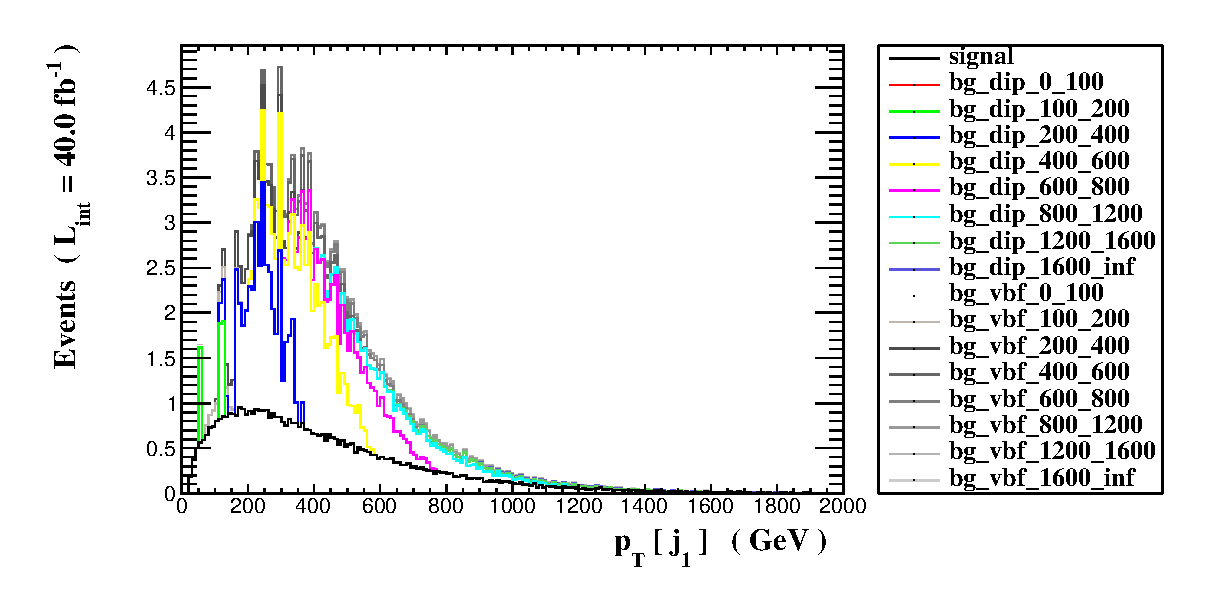
\includegraphics[scale=0.45]{selection_0.eps}\\
\caption{   }
  \end{center}
\end{figure}
      \newpage
\subsection{ Histogram 2}

\textbf{* Plot: ETA ( jets[1] ) }\\
   \begin{table}[H]
  \begin{center}
    \begin{tabular}{|m{23.0mm}|m{23.0mm}|m{18.0mm}|m{19.0mm}|m{19.0mm}|m{19.0mm}|m{19.0mm}|}
      \hline
      {\cellcolor{yellow}         Dataset}& {\cellcolor{yellow}         Integral}& {\cellcolor{yellow}         Entries per event}& {\cellcolor{yellow}         Mean}& {\cellcolor{yellow}         RMS}& {\cellcolor{yellow}         \% underflow}& {\cellcolor{yellow}         \% overflow}\\
      \hline
      {\cellcolor{white}         signal}& {\cellcolor{white}         52.9}& {\cellcolor{white}         1.0}& {\cellcolor{white}         -0.00747599}& {\cellcolor{white}         1.887}& {\cellcolor{green}         0.0}& {\cellcolor{green}         0.0}\\
      \hline
      {\cellcolor{white}         bg\_dip\_0\_100}& {\cellcolor{white}         0.0 +/\-- 0.0}& {\cellcolor{white}         0.}& {\cellcolor{white}         0.0}& {\cellcolor{white}         0.0}& {\cellcolor{green}         0.0}& {\cellcolor{green}         0.0}\\
      \hline
      {\cellcolor{white}         bg\_dip\_100\_200}& {\cellcolor{white}         3.16}& {\cellcolor{white}         1.0}& {\cellcolor{white}         1.65038}& {\cellcolor{white}         2.73}& {\cellcolor{green}         0.0}& {\cellcolor{green}         0.0}\\
      \hline
      {\cellcolor{white}         bg\_dip\_200\_400}& {\cellcolor{white}         25.8}& {\cellcolor{white}         1.0}& {\cellcolor{white}         0.0327822}& {\cellcolor{white}         1.622}& {\cellcolor{green}         0.0}& {\cellcolor{green}         0.0}\\
      \hline
      {\cellcolor{white}         bg\_dip\_400\_600}& {\cellcolor{white}         34.8}& {\cellcolor{white}         1.0}& {\cellcolor{white}         0.0508046}& {\cellcolor{white}         1.367}& {\cellcolor{green}         0.0}& {\cellcolor{green}         0.0}\\
      \hline
      {\cellcolor{white}         bg\_dip\_600\_800}& {\cellcolor{white}         18.8}& {\cellcolor{white}         1.0}& {\cellcolor{white}         -0.0541901}& {\cellcolor{white}         1.213}& {\cellcolor{green}         0.0}& {\cellcolor{green}         0.0}\\
      \hline
      {\cellcolor{white}         bg\_dip\_800\_1200}& {\cellcolor{white}         11.4}& {\cellcolor{white}         1.0}& {\cellcolor{white}         0.00988796}& {\cellcolor{white}         1.116}& {\cellcolor{green}         0.0}& {\cellcolor{green}         0.0}\\
      \hline
      {\cellcolor{white}         bg\_dip\_1200\_1600}& {\cellcolor{white}         1.92}& {\cellcolor{white}         1.0}& {\cellcolor{white}         -0.041622}& {\cellcolor{white}         1.098}& {\cellcolor{green}         0.0}& {\cellcolor{green}         0.0}\\
      \hline
      {\cellcolor{white}         bg\_dip\_1600\_inf}& {\cellcolor{white}         0.492}& {\cellcolor{white}         1.0}& {\cellcolor{white}         0.0236354}& {\cellcolor{white}         1.091}& {\cellcolor{green}         0.0}& {\cellcolor{green}         0.0}\\
      \hline
      {\cellcolor{white}         bg\_vbf\_0\_100}& {\cellcolor{white}         0.0486}& {\cellcolor{white}         1.0}& {\cellcolor{white}         0.873486}& {\cellcolor{white}         2.934}& {\cellcolor{green}         0.0}& {\cellcolor{green}         0.0}\\
      \hline
      {\cellcolor{white}         bg\_vbf\_100\_200}& {\cellcolor{white}         1.16}& {\cellcolor{white}         1.0}& {\cellcolor{white}         0.133336}& {\cellcolor{white}         2.773}& {\cellcolor{green}         0.0}& {\cellcolor{green}         0.0}\\
      \hline
      {\cellcolor{white}         bg\_vbf\_200\_400}& {\cellcolor{white}         6.68}& {\cellcolor{white}         1.0}& {\cellcolor{white}         0.0158882}& {\cellcolor{white}         2.195}& {\cellcolor{green}         0.0}& {\cellcolor{green}         0.0}\\
      \hline
      {\cellcolor{white}         bg\_vbf\_400\_600}& {\cellcolor{white}         7.09}& {\cellcolor{white}         1.0}& {\cellcolor{white}         -0.0150998}& {\cellcolor{white}         1.768}& {\cellcolor{green}         0.0}& {\cellcolor{green}         0.0}\\
      \hline
      {\cellcolor{white}         bg\_vbf\_600\_800}& {\cellcolor{white}         3.66}& {\cellcolor{white}         1.0}& {\cellcolor{white}         -9.49209e-06}& {\cellcolor{white}         1.521}& {\cellcolor{green}         0.0}& {\cellcolor{green}         0.0}\\
      \hline
      {\cellcolor{white}         bg\_vbf\_800\_1200}& {\cellcolor{white}         2.15}& {\cellcolor{white}         1.0}& {\cellcolor{white}         -0.0314427}& {\cellcolor{white}         1.333}& {\cellcolor{green}         0.0}& {\cellcolor{green}         0.0}\\
      \hline
      {\cellcolor{white}         bg\_vbf\_1200\_1600}& {\cellcolor{white}         0.385}& {\cellcolor{white}         1.0}& {\cellcolor{white}         -0.015205}& {\cellcolor{white}         1.192}& {\cellcolor{green}         0.0}& {\cellcolor{green}         0.0}\\
      \hline
      {\cellcolor{white}         bg\_vbf\_1600\_inf}& {\cellcolor{white}         0.0982}& {\cellcolor{white}         1.0}& {\cellcolor{white}         0.026085}& {\cellcolor{white}         1.094}& {\cellcolor{green}         0.0}& {\cellcolor{green}         0.0}\\
\hline
    \end{tabular}
  \end{center}
\end{table}

\begin{figure}[H]
  \begin{center}
    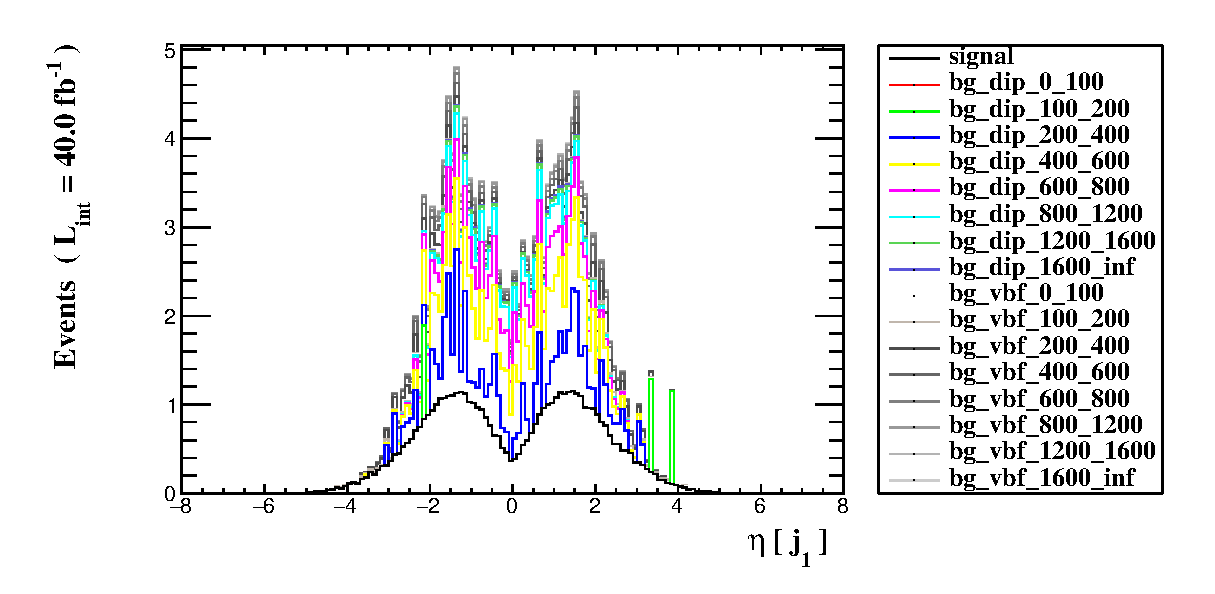
\includegraphics[scale=0.45]{selection_1.eps}\\
\caption{   }
  \end{center}
\end{figure}
      \newpage
\subsection{ Histogram 3}

\textbf{* Plot: PHI ( jets[1] ) }\\
   \begin{table}[H]
  \begin{center}
    \begin{tabular}{|m{23.0mm}|m{23.0mm}|m{18.0mm}|m{19.0mm}|m{19.0mm}|m{19.0mm}|m{19.0mm}|}
      \hline
      {\cellcolor{yellow}         Dataset}& {\cellcolor{yellow}         Integral}& {\cellcolor{yellow}         Entries per event}& {\cellcolor{yellow}         Mean}& {\cellcolor{yellow}         RMS}& {\cellcolor{yellow}         \% underflow}& {\cellcolor{yellow}         \% overflow}\\
      \hline
      {\cellcolor{white}         signal}& {\cellcolor{white}         52.9}& {\cellcolor{white}         1.0}& {\cellcolor{white}         0.00275702}& {\cellcolor{white}         1.825}& {\cellcolor{green}         0.0}& {\cellcolor{green}         0.0}\\
      \hline
      {\cellcolor{white}         bg\_dip\_0\_100}& {\cellcolor{white}         0.0 +/\-- 0.0}& {\cellcolor{white}         0.}& {\cellcolor{white}         0.0}& {\cellcolor{white}         0.0}& {\cellcolor{green}         0.0}& {\cellcolor{green}         0.0}\\
      \hline
      {\cellcolor{white}         bg\_dip\_100\_200}& {\cellcolor{white}         3.16}& {\cellcolor{white}         1.0}& {\cellcolor{white}         0.466209}& {\cellcolor{white}         0.3607}& {\cellcolor{green}         0.0}& {\cellcolor{green}         0.0}\\
      \hline
      {\cellcolor{white}         bg\_dip\_200\_400}& {\cellcolor{white}         25.8}& {\cellcolor{white}         1.0}& {\cellcolor{white}         -0.0184691}& {\cellcolor{white}         1.809}& {\cellcolor{green}         0.0}& {\cellcolor{green}         0.0}\\
      \hline
      {\cellcolor{white}         bg\_dip\_400\_600}& {\cellcolor{white}         34.8}& {\cellcolor{white}         1.0}& {\cellcolor{white}         -0.032295}& {\cellcolor{white}         1.807}& {\cellcolor{green}         0.0}& {\cellcolor{green}         0.0}\\
      \hline
      {\cellcolor{white}         bg\_dip\_600\_800}& {\cellcolor{white}         18.8}& {\cellcolor{white}         1.0}& {\cellcolor{white}         0.0217009}& {\cellcolor{white}         1.85}& {\cellcolor{green}         0.0}& {\cellcolor{green}         0.0}\\
      \hline
      {\cellcolor{white}         bg\_dip\_800\_1200}& {\cellcolor{white}         11.4}& {\cellcolor{white}         1.0}& {\cellcolor{white}         -0.0214499}& {\cellcolor{white}         1.813}& {\cellcolor{green}         0.0}& {\cellcolor{green}         0.0}\\
      \hline
      {\cellcolor{white}         bg\_dip\_1200\_1600}& {\cellcolor{white}         1.92}& {\cellcolor{white}         1.0}& {\cellcolor{white}         -0.0349831}& {\cellcolor{white}         1.831}& {\cellcolor{green}         0.0}& {\cellcolor{green}         0.0}\\
      \hline
      {\cellcolor{white}         bg\_dip\_1600\_inf}& {\cellcolor{white}         0.492}& {\cellcolor{white}         1.0}& {\cellcolor{white}         -0.0245294}& {\cellcolor{white}         1.837}& {\cellcolor{green}         0.0}& {\cellcolor{green}         0.0}\\
      \hline
      {\cellcolor{white}         bg\_vbf\_0\_100}& {\cellcolor{white}         0.0486}& {\cellcolor{white}         1.0}& {\cellcolor{white}         -0.168141}& {\cellcolor{white}         1.997}& {\cellcolor{green}         0.0}& {\cellcolor{green}         0.0}\\
      \hline
      {\cellcolor{white}         bg\_vbf\_100\_200}& {\cellcolor{white}         1.16}& {\cellcolor{white}         1.0}& {\cellcolor{white}         -0.0767497}& {\cellcolor{white}         1.778}& {\cellcolor{green}         0.0}& {\cellcolor{green}         0.0}\\
      \hline
      {\cellcolor{white}         bg\_vbf\_200\_400}& {\cellcolor{white}         6.68}& {\cellcolor{white}         1.0}& {\cellcolor{white}         -0.0861787}& {\cellcolor{white}         1.817}& {\cellcolor{green}         0.0}& {\cellcolor{green}         0.0}\\
      \hline
      {\cellcolor{white}         bg\_vbf\_400\_600}& {\cellcolor{white}         7.09}& {\cellcolor{white}         1.0}& {\cellcolor{white}         0.0245695}& {\cellcolor{white}         1.804}& {\cellcolor{green}         0.0}& {\cellcolor{green}         0.0}\\
      \hline
      {\cellcolor{white}         bg\_vbf\_600\_800}& {\cellcolor{white}         3.66}& {\cellcolor{white}         1.0}& {\cellcolor{white}         0.0164854}& {\cellcolor{white}         1.806}& {\cellcolor{green}         0.0}& {\cellcolor{green}         0.0}\\
      \hline
      {\cellcolor{white}         bg\_vbf\_800\_1200}& {\cellcolor{white}         2.15}& {\cellcolor{white}         1.0}& {\cellcolor{white}         0.0186246}& {\cellcolor{white}         1.811}& {\cellcolor{green}         0.0}& {\cellcolor{green}         0.0}\\
      \hline
      {\cellcolor{white}         bg\_vbf\_1200\_1600}& {\cellcolor{white}         0.385}& {\cellcolor{white}         1.0}& {\cellcolor{white}         0.0173015}& {\cellcolor{white}         1.812}& {\cellcolor{green}         0.0}& {\cellcolor{green}         0.0}\\
      \hline
      {\cellcolor{white}         bg\_vbf\_1600\_inf}& {\cellcolor{white}         0.0982}& {\cellcolor{white}         1.0}& {\cellcolor{white}         0.0489667}& {\cellcolor{white}         1.807}& {\cellcolor{green}         0.0}& {\cellcolor{green}         0.0}\\
\hline
    \end{tabular}
  \end{center}
\end{table}

\begin{figure}[H]
  \begin{center}
    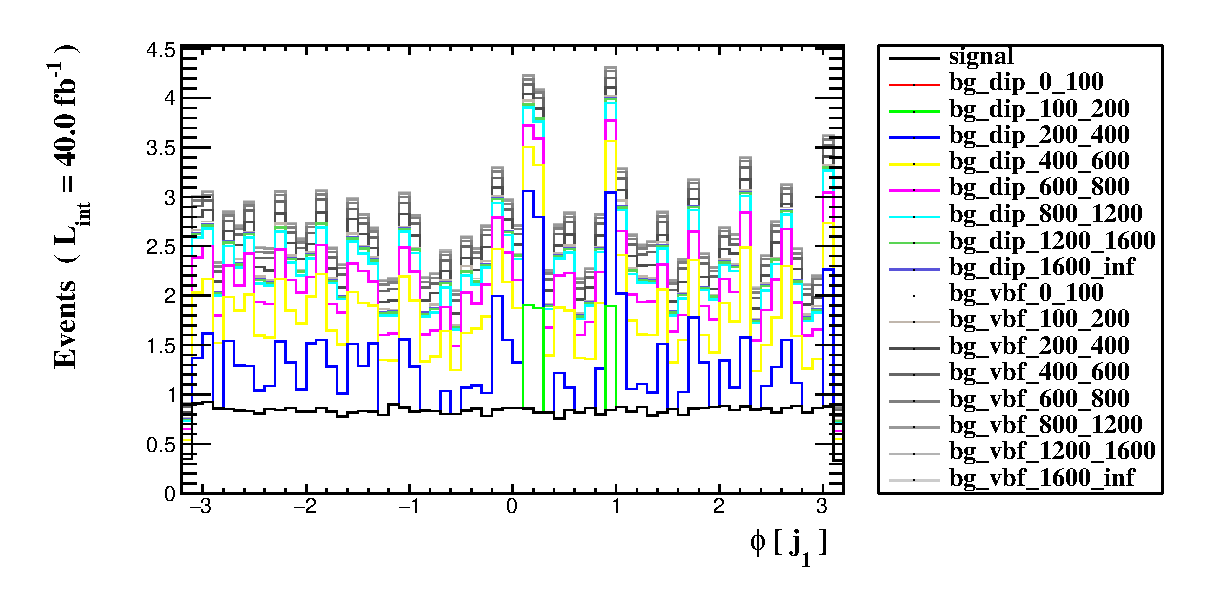
\includegraphics[scale=0.45]{selection_2.eps}\\
\caption{   }
  \end{center}
\end{figure}
      \newpage
\subsection{ Histogram 4}

\textbf{* Plot: PT ( jets[2] ) }\\
   \begin{table}[H]
  \begin{center}
    \begin{tabular}{|m{23.0mm}|m{23.0mm}|m{18.0mm}|m{19.0mm}|m{19.0mm}|m{19.0mm}|m{19.0mm}|}
      \hline
      {\cellcolor{yellow}         Dataset}& {\cellcolor{yellow}         Integral}& {\cellcolor{yellow}         Entries per event}& {\cellcolor{yellow}         Mean}& {\cellcolor{yellow}         RMS}& {\cellcolor{yellow}         \% underflow}& {\cellcolor{yellow}         \% overflow}\\
      \hline
      {\cellcolor{white}         signal}& {\cellcolor{white}         52.9}& {\cellcolor{white}         1.0}& {\cellcolor{white}         149.999}& {\cellcolor{white}         130.2}& {\cellcolor{green}         0.0}& {\cellcolor{green}         0.05862}\\
      \hline
      {\cellcolor{white}         bg\_dip\_0\_100}& {\cellcolor{white}         0.0 +/\-- 0.0}& {\cellcolor{white}         0.}& {\cellcolor{white}         0.0}& {\cellcolor{white}         0.0}& {\cellcolor{green}         0.0}& {\cellcolor{green}         0.0}\\
      \hline
      {\cellcolor{white}         bg\_dip\_100\_200}& {\cellcolor{white}         3.16}& {\cellcolor{white}         1.0}& {\cellcolor{white}         49.3379}& {\cellcolor{white}         16.83}& {\cellcolor{green}         0.0}& {\cellcolor{green}         0.0}\\
      \hline
      {\cellcolor{white}         bg\_dip\_200\_400}& {\cellcolor{white}         25.8}& {\cellcolor{white}         1.0}& {\cellcolor{white}         80.1038}& {\cellcolor{white}         38.82}& {\cellcolor{green}         0.0}& {\cellcolor{green}         0.0}\\
      \hline
      {\cellcolor{white}         bg\_dip\_400\_600}& {\cellcolor{white}         34.8}& {\cellcolor{white}         1.0}& {\cellcolor{white}         120.487}& {\cellcolor{white}         64.78}& {\cellcolor{green}         0.0}& {\cellcolor{green}         0.0}\\
      \hline
      {\cellcolor{white}         bg\_dip\_600\_800}& {\cellcolor{white}         18.8}& {\cellcolor{white}         1.0}& {\cellcolor{white}         164.154}& {\cellcolor{white}         90.7}& {\cellcolor{green}         0.0}& {\cellcolor{green}         0.0}\\
      \hline
      {\cellcolor{white}         bg\_dip\_800\_1200}& {\cellcolor{white}         11.4}& {\cellcolor{white}         1.0}& {\cellcolor{white}         229.974}& {\cellcolor{white}         135.8}& {\cellcolor{green}         0.0}& {\cellcolor{green}         0.0}\\
      \hline
      {\cellcolor{white}         bg\_dip\_1200\_1600}& {\cellcolor{white}         1.92}& {\cellcolor{white}         1.0}& {\cellcolor{white}         373.02}& {\cellcolor{white}         205.5}& {\cellcolor{green}         0.0}& {\cellcolor{green}         0.0}\\
      \hline
      {\cellcolor{white}         bg\_dip\_1600\_inf}& {\cellcolor{white}         0.492}& {\cellcolor{white}         1.0}& {\cellcolor{white}         650.81}& {\cellcolor{white}         284.8}& {\cellcolor{orange}         0.0}& {\cellcolor{orange}         7.302}\\
      \hline
      {\cellcolor{white}         bg\_vbf\_0\_100}& {\cellcolor{white}         0.0486}& {\cellcolor{white}         1.0}& {\cellcolor{white}         31.916}& {\cellcolor{white}         8.29}& {\cellcolor{green}         0.0}& {\cellcolor{green}         0.0}\\
      \hline
      {\cellcolor{white}         bg\_vbf\_100\_200}& {\cellcolor{white}         1.16}& {\cellcolor{white}         1.0}& {\cellcolor{white}         53.936}& {\cellcolor{white}         17.53}& {\cellcolor{green}         0.0}& {\cellcolor{green}         0.0}\\
      \hline
      {\cellcolor{white}         bg\_vbf\_200\_400}& {\cellcolor{white}         6.68}& {\cellcolor{white}         1.0}& {\cellcolor{white}         94.1307}& {\cellcolor{white}         38.71}& {\cellcolor{green}         0.0}& {\cellcolor{green}         0.0}\\
      \hline
      {\cellcolor{white}         bg\_vbf\_400\_600}& {\cellcolor{white}         7.09}& {\cellcolor{white}         1.0}& {\cellcolor{white}         136.14}& {\cellcolor{white}         60.57}& {\cellcolor{green}         0.0}& {\cellcolor{green}         0.0}\\
      \hline
      {\cellcolor{white}         bg\_vbf\_600\_800}& {\cellcolor{white}         3.66}& {\cellcolor{white}         1.0}& {\cellcolor{white}         186.868}& {\cellcolor{white}         85.24}& {\cellcolor{green}         0.0}& {\cellcolor{green}         0.0}\\
      \hline
      {\cellcolor{white}         bg\_vbf\_800\_1200}& {\cellcolor{white}         2.15}& {\cellcolor{white}         1.0}& {\cellcolor{white}         257.298}& {\cellcolor{white}         127.5}& {\cellcolor{green}         0.0}& {\cellcolor{green}         0.0}\\
      \hline
      {\cellcolor{white}         bg\_vbf\_1200\_1600}& {\cellcolor{white}         0.385}& {\cellcolor{white}         1.0}& {\cellcolor{white}         392.815}& {\cellcolor{white}         188.0}& {\cellcolor{green}         0.0}& {\cellcolor{green}         0.0}\\
      \hline
      {\cellcolor{white}         bg\_vbf\_1600\_inf}& {\cellcolor{white}         0.0982}& {\cellcolor{white}         1.0}& {\cellcolor{white}         599.859}& {\cellcolor{white}         284.3}& {\cellcolor{orange}         0.0}& {\cellcolor{orange}         5.572}\\
\hline
    \end{tabular}
  \end{center}
\end{table}

\begin{figure}[H]
  \begin{center}
    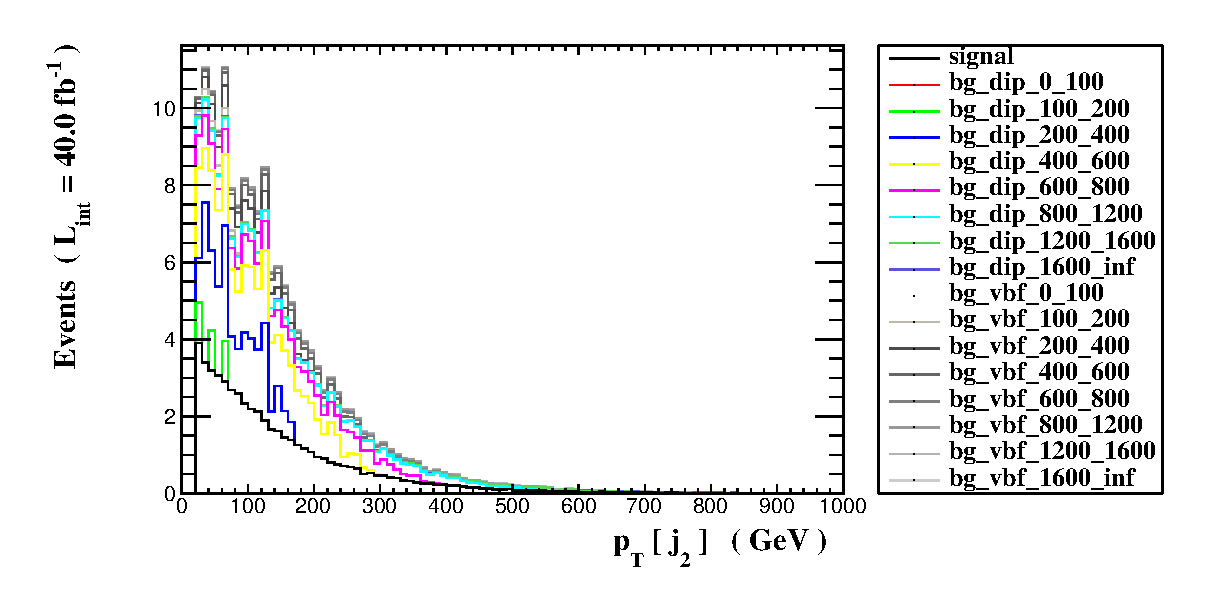
\includegraphics[scale=0.45]{selection_3.eps}\\
\caption{   }
  \end{center}
\end{figure}
      \newpage
\subsection{ Histogram 5}

\textbf{* Plot: ETA ( jets[2] ) }\\
   \begin{table}[H]
  \begin{center}
    \begin{tabular}{|m{23.0mm}|m{23.0mm}|m{18.0mm}|m{19.0mm}|m{19.0mm}|m{19.0mm}|m{19.0mm}|}
      \hline
      {\cellcolor{yellow}         Dataset}& {\cellcolor{yellow}         Integral}& {\cellcolor{yellow}         Entries per event}& {\cellcolor{yellow}         Mean}& {\cellcolor{yellow}         RMS}& {\cellcolor{yellow}         \% underflow}& {\cellcolor{yellow}         \% overflow}\\
      \hline
      {\cellcolor{white}         signal}& {\cellcolor{white}         52.9}& {\cellcolor{white}         1.0}& {\cellcolor{white}         -0.00789021}& {\cellcolor{white}         2.717}& {\cellcolor{green}         0.0}& {\cellcolor{green}         0.0}\\
      \hline
      {\cellcolor{white}         bg\_dip\_0\_100}& {\cellcolor{white}         0.0 +/\-- 0.0}& {\cellcolor{white}         0.}& {\cellcolor{white}         0.0}& {\cellcolor{white}         0.0}& {\cellcolor{green}         0.0}& {\cellcolor{green}         0.0}\\
      \hline
      {\cellcolor{white}         bg\_dip\_100\_200}& {\cellcolor{white}         3.16}& {\cellcolor{white}         1.0}& {\cellcolor{white}         0.140052}& {\cellcolor{white}         2.918}& {\cellcolor{green}         0.0}& {\cellcolor{green}         0.0}\\
      \hline
      {\cellcolor{white}         bg\_dip\_200\_400}& {\cellcolor{white}         25.8}& {\cellcolor{white}         1.0}& {\cellcolor{white}         0.341283}& {\cellcolor{white}         2.913}& {\cellcolor{green}         0.0}& {\cellcolor{green}         0.0}\\
      \hline
      {\cellcolor{white}         bg\_dip\_400\_600}& {\cellcolor{white}         34.8}& {\cellcolor{white}         1.0}& {\cellcolor{white}         -0.046237}& {\cellcolor{white}         2.471}& {\cellcolor{green}         0.0}& {\cellcolor{green}         0.0}\\
      \hline
      {\cellcolor{white}         bg\_dip\_600\_800}& {\cellcolor{white}         18.8}& {\cellcolor{white}         1.0}& {\cellcolor{white}         0.0328972}& {\cellcolor{white}         2.251}& {\cellcolor{green}         0.0}& {\cellcolor{green}         0.0}\\
      \hline
      {\cellcolor{white}         bg\_dip\_800\_1200}& {\cellcolor{white}         11.4}& {\cellcolor{white}         1.0}& {\cellcolor{white}         -0.0295072}& {\cellcolor{white}         2.126}& {\cellcolor{green}         0.0}& {\cellcolor{green}         0.0}\\
      \hline
      {\cellcolor{white}         bg\_dip\_1200\_1600}& {\cellcolor{white}         1.92}& {\cellcolor{white}         1.0}& {\cellcolor{white}         -0.00220058}& {\cellcolor{white}         1.896}& {\cellcolor{green}         0.0}& {\cellcolor{green}         0.0}\\
      \hline
      {\cellcolor{white}         bg\_dip\_1600\_inf}& {\cellcolor{white}         0.492}& {\cellcolor{white}         1.0}& {\cellcolor{white}         -0.0593366}& {\cellcolor{white}         1.605}& {\cellcolor{green}         0.0}& {\cellcolor{green}         0.0}\\
      \hline
      {\cellcolor{white}         bg\_vbf\_0\_100}& {\cellcolor{white}         0.0486}& {\cellcolor{white}         1.0}& {\cellcolor{white}         1.04772}& {\cellcolor{white}         3.507}& {\cellcolor{green}         0.0}& {\cellcolor{green}         0.0}\\
      \hline
      {\cellcolor{white}         bg\_vbf\_100\_200}& {\cellcolor{white}         1.16}& {\cellcolor{white}         1.0}& {\cellcolor{white}         -0.324417}& {\cellcolor{white}         3.174}& {\cellcolor{green}         0.0}& {\cellcolor{green}         0.0}\\
      \hline
      {\cellcolor{white}         bg\_vbf\_200\_400}& {\cellcolor{white}         6.68}& {\cellcolor{white}         1.0}& {\cellcolor{white}         0.0369757}& {\cellcolor{white}         2.866}& {\cellcolor{green}         0.0}& {\cellcolor{green}         0.0}\\
      \hline
      {\cellcolor{white}         bg\_vbf\_400\_600}& {\cellcolor{white}         7.09}& {\cellcolor{white}         1.0}& {\cellcolor{white}         0.0457121}& {\cellcolor{white}         2.548}& {\cellcolor{green}         0.0}& {\cellcolor{green}         0.0}\\
      \hline
      {\cellcolor{white}         bg\_vbf\_600\_800}& {\cellcolor{white}         3.66}& {\cellcolor{white}         1.0}& {\cellcolor{white}         0.00762408}& {\cellcolor{white}         2.33}& {\cellcolor{green}         0.0}& {\cellcolor{green}         0.0}\\
      \hline
      {\cellcolor{white}         bg\_vbf\_800\_1200}& {\cellcolor{white}         2.15}& {\cellcolor{white}         1.0}& {\cellcolor{white}         0.0416591}& {\cellcolor{white}         2.175}& {\cellcolor{green}         0.0}& {\cellcolor{green}         0.0}\\
      \hline
      {\cellcolor{white}         bg\_vbf\_1200\_1600}& {\cellcolor{white}         0.385}& {\cellcolor{white}         1.0}& {\cellcolor{white}         0.0257553}& {\cellcolor{white}         1.974}& {\cellcolor{green}         0.0}& {\cellcolor{green}         0.0}\\
      \hline
      {\cellcolor{white}         bg\_vbf\_1600\_inf}& {\cellcolor{white}         0.0982}& {\cellcolor{white}         1.0}& {\cellcolor{white}         -0.0204758}& {\cellcolor{white}         1.781}& {\cellcolor{green}         0.0}& {\cellcolor{green}         0.0}\\
\hline
    \end{tabular}
  \end{center}
\end{table}

\begin{figure}[H]
  \begin{center}
    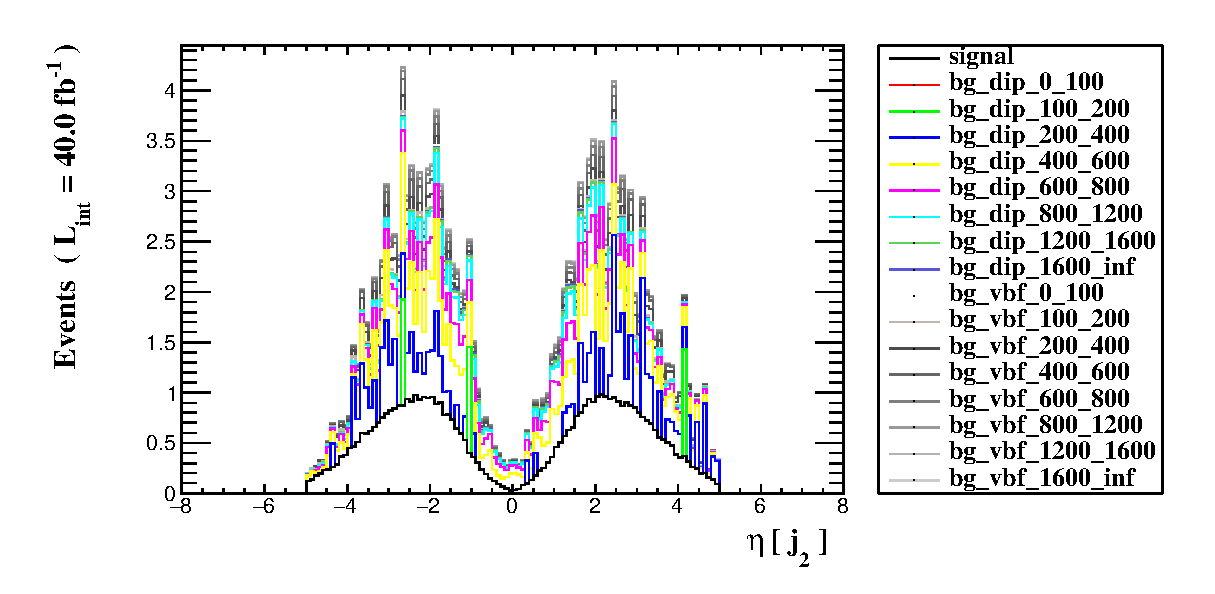
\includegraphics[scale=0.45]{selection_4.eps}\\
\caption{   }
  \end{center}
\end{figure}
      \newpage
\subsection{ Histogram 6}

\textbf{* Plot: PHI ( jets[2] ) }\\
   \begin{table}[H]
  \begin{center}
    \begin{tabular}{|m{23.0mm}|m{23.0mm}|m{18.0mm}|m{19.0mm}|m{19.0mm}|m{19.0mm}|m{19.0mm}|}
      \hline
      {\cellcolor{yellow}         Dataset}& {\cellcolor{yellow}         Integral}& {\cellcolor{yellow}         Entries per event}& {\cellcolor{yellow}         Mean}& {\cellcolor{yellow}         RMS}& {\cellcolor{yellow}         \% underflow}& {\cellcolor{yellow}         \% overflow}\\
      \hline
      {\cellcolor{white}         signal}& {\cellcolor{white}         52.9}& {\cellcolor{white}         1.0}& {\cellcolor{white}         -0.00536837}& {\cellcolor{white}         1.814}& {\cellcolor{green}         0.0}& {\cellcolor{green}         0.0}\\
      \hline
      {\cellcolor{white}         bg\_dip\_0\_100}& {\cellcolor{white}         0.0 +/\-- 0.0}& {\cellcolor{white}         0.}& {\cellcolor{white}         0.0}& {\cellcolor{white}         0.0}& {\cellcolor{green}         0.0}& {\cellcolor{green}         0.0}\\
      \hline
      {\cellcolor{white}         bg\_dip\_100\_200}& {\cellcolor{white}         3.16}& {\cellcolor{white}         1.0}& {\cellcolor{white}         1.00733}& {\cellcolor{white}         1.634}& {\cellcolor{green}         0.0}& {\cellcolor{green}         0.0}\\
      \hline
      {\cellcolor{white}         bg\_dip\_200\_400}& {\cellcolor{white}         25.8}& {\cellcolor{white}         1.0}& {\cellcolor{white}         -0.0150701}& {\cellcolor{white}         1.924}& {\cellcolor{green}         0.0}& {\cellcolor{green}         0.0}\\
      \hline
      {\cellcolor{white}         bg\_dip\_400\_600}& {\cellcolor{white}         34.8}& {\cellcolor{white}         1.0}& {\cellcolor{white}         -0.0100722}& {\cellcolor{white}         1.806}& {\cellcolor{green}         0.0}& {\cellcolor{green}         0.0}\\
      \hline
      {\cellcolor{white}         bg\_dip\_600\_800}& {\cellcolor{white}         18.8}& {\cellcolor{white}         1.0}& {\cellcolor{white}         0.0584177}& {\cellcolor{white}         1.785}& {\cellcolor{green}         0.0}& {\cellcolor{green}         0.0}\\
      \hline
      {\cellcolor{white}         bg\_dip\_800\_1200}& {\cellcolor{white}         11.4}& {\cellcolor{white}         1.0}& {\cellcolor{white}         0.0255093}& {\cellcolor{white}         1.793}& {\cellcolor{green}         0.0}& {\cellcolor{green}         0.0}\\
      \hline
      {\cellcolor{white}         bg\_dip\_1200\_1600}& {\cellcolor{white}         1.92}& {\cellcolor{white}         1.0}& {\cellcolor{white}         -0.000600709}& {\cellcolor{white}         1.8}& {\cellcolor{green}         0.0}& {\cellcolor{green}         0.0}\\
      \hline
      {\cellcolor{white}         bg\_dip\_1600\_inf}& {\cellcolor{white}         0.492}& {\cellcolor{white}         1.0}& {\cellcolor{white}         -0.0251717}& {\cellcolor{white}         1.798}& {\cellcolor{green}         0.0}& {\cellcolor{green}         0.0}\\
      \hline
      {\cellcolor{white}         bg\_vbf\_0\_100}& {\cellcolor{white}         0.0486}& {\cellcolor{white}         1.0}& {\cellcolor{white}         0.0859607}& {\cellcolor{white}         1.498}& {\cellcolor{green}         0.0}& {\cellcolor{green}         0.0}\\
      \hline
      {\cellcolor{white}         bg\_vbf\_100\_200}& {\cellcolor{white}         1.16}& {\cellcolor{white}         1.0}& {\cellcolor{white}         0.17327}& {\cellcolor{white}         1.879}& {\cellcolor{green}         0.0}& {\cellcolor{green}         0.0}\\
      \hline
      {\cellcolor{white}         bg\_vbf\_200\_400}& {\cellcolor{white}         6.68}& {\cellcolor{white}         1.0}& {\cellcolor{white}         -0.0623337}& {\cellcolor{white}         1.832}& {\cellcolor{green}         0.0}& {\cellcolor{green}         0.0}\\
      \hline
      {\cellcolor{white}         bg\_vbf\_400\_600}& {\cellcolor{white}         7.09}& {\cellcolor{white}         1.0}& {\cellcolor{white}         -0.0408524}& {\cellcolor{white}         1.826}& {\cellcolor{green}         0.0}& {\cellcolor{green}         0.0}\\
      \hline
      {\cellcolor{white}         bg\_vbf\_600\_800}& {\cellcolor{white}         3.66}& {\cellcolor{white}         1.0}& {\cellcolor{white}         -0.0166052}& {\cellcolor{white}         1.814}& {\cellcolor{green}         0.0}& {\cellcolor{green}         0.0}\\
      \hline
      {\cellcolor{white}         bg\_vbf\_800\_1200}& {\cellcolor{white}         2.15}& {\cellcolor{white}         1.0}& {\cellcolor{white}         -0.0206916}& {\cellcolor{white}         1.807}& {\cellcolor{green}         0.0}& {\cellcolor{green}         0.0}\\
      \hline
      {\cellcolor{white}         bg\_vbf\_1200\_1600}& {\cellcolor{white}         0.385}& {\cellcolor{white}         1.0}& {\cellcolor{white}         -0.0182899}& {\cellcolor{white}         1.813}& {\cellcolor{green}         0.0}& {\cellcolor{green}         0.0}\\
      \hline
      {\cellcolor{white}         bg\_vbf\_1600\_inf}& {\cellcolor{white}         0.0982}& {\cellcolor{white}         1.0}& {\cellcolor{white}         0.00781695}& {\cellcolor{white}         1.811}& {\cellcolor{green}         0.0}& {\cellcolor{green}         0.0}\\
\hline
    \end{tabular}
  \end{center}
\end{table}

\begin{figure}[H]
  \begin{center}
    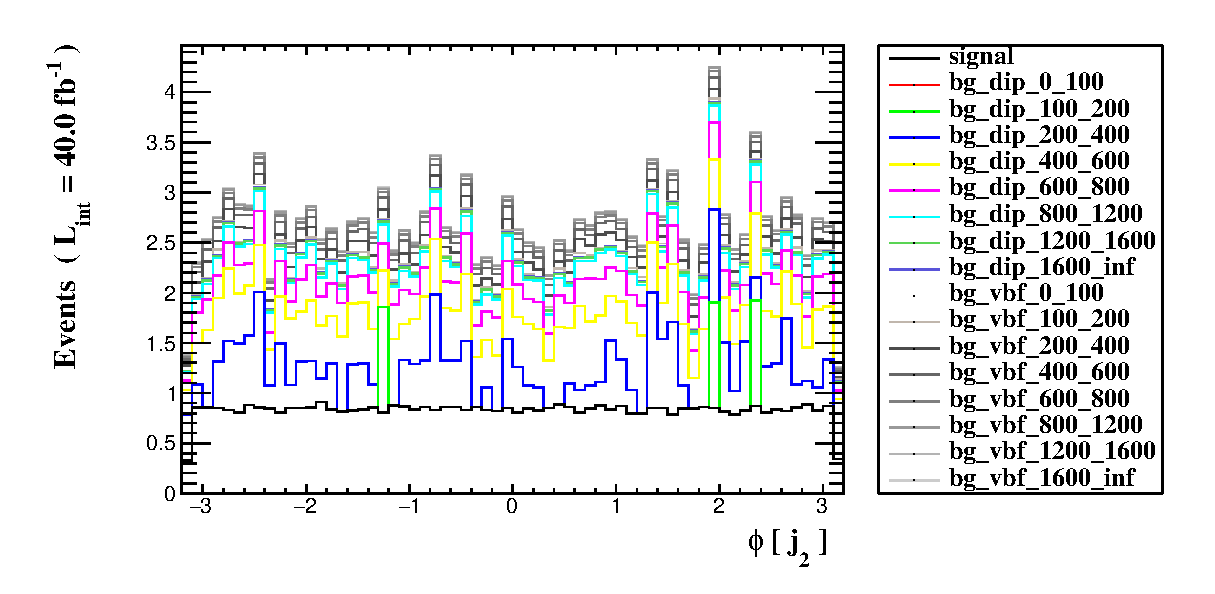
\includegraphics[scale=0.45]{selection_5.eps}\\
\caption{   }
  \end{center}
\end{figure}
      \newpage
\subsection{ Histogram 7}

\textbf{* Plot: DELTAR ( jets[1] , jets[2] ) }\\
   \begin{table}[H]
  \begin{center}
    \begin{tabular}{|m{23.0mm}|m{23.0mm}|m{18.0mm}|m{19.0mm}|m{19.0mm}|m{19.0mm}|m{19.0mm}|}
      \hline
      {\cellcolor{yellow}         Dataset}& {\cellcolor{yellow}         Integral}& {\cellcolor{yellow}         Entries per event}& {\cellcolor{yellow}         Mean}& {\cellcolor{yellow}         RMS}& {\cellcolor{yellow}         \% underflow}& {\cellcolor{yellow}         \% overflow}\\
      \hline
      {\cellcolor{white}         signal}& {\cellcolor{white}         52.9}& {\cellcolor{white}         1.0}& {\cellcolor{white}         4.56273}& {\cellcolor{white}         1.361}& {\cellcolor{green}         0.0}& {\cellcolor{green}         0.0}\\
      \hline
      {\cellcolor{white}         bg\_dip\_0\_100}& {\cellcolor{white}         0.0 +/\-- 0.0}& {\cellcolor{white}         0.}& {\cellcolor{white}         0.0}& {\cellcolor{white}         0.0}& {\cellcolor{green}         0.0}& {\cellcolor{green}         0.0}\\
      \hline
      {\cellcolor{white}         bg\_dip\_100\_200}& {\cellcolor{white}         3.16}& {\cellcolor{white}         1.0}& {\cellcolor{white}         5.99929}& {\cellcolor{white}         0.4811}& {\cellcolor{green}         0.0}& {\cellcolor{green}         0.0}\\
      \hline
      {\cellcolor{white}         bg\_dip\_200\_400}& {\cellcolor{white}         25.8}& {\cellcolor{white}         1.0}& {\cellcolor{white}         4.61504}& {\cellcolor{white}         0.7198}& {\cellcolor{green}         0.0}& {\cellcolor{green}         0.0}\\
      \hline
      {\cellcolor{white}         bg\_dip\_400\_600}& {\cellcolor{white}         34.8}& {\cellcolor{white}         1.0}& {\cellcolor{white}         3.97985}& {\cellcolor{white}         0.723}& {\cellcolor{green}         0.0}& {\cellcolor{green}         0.0}\\
      \hline
      {\cellcolor{white}         bg\_dip\_600\_800}& {\cellcolor{white}         18.8}& {\cellcolor{white}         1.0}& {\cellcolor{white}         3.73769}& {\cellcolor{white}         0.6876}& {\cellcolor{green}         0.0}& {\cellcolor{green}         0.0}\\
      \hline
      {\cellcolor{white}         bg\_dip\_800\_1200}& {\cellcolor{white}         11.4}& {\cellcolor{white}         1.0}& {\cellcolor{white}         3.67888}& {\cellcolor{white}         0.627}& {\cellcolor{green}         0.0}& {\cellcolor{green}         0.0}\\
      \hline
      {\cellcolor{white}         bg\_dip\_1200\_1600}& {\cellcolor{white}         1.92}& {\cellcolor{white}         1.0}& {\cellcolor{white}         3.64813}& {\cellcolor{white}         0.5268}& {\cellcolor{green}         0.0}& {\cellcolor{green}         0.0}\\
      \hline
      {\cellcolor{white}         bg\_dip\_1600\_inf}& {\cellcolor{white}         0.492}& {\cellcolor{white}         1.0}& {\cellcolor{white}         3.64692}& {\cellcolor{white}         0.4106}& {\cellcolor{green}         0.0}& {\cellcolor{green}         0.0}\\
      \hline
      {\cellcolor{white}         bg\_vbf\_0\_100}& {\cellcolor{white}         0.0486}& {\cellcolor{white}         1.0}& {\cellcolor{white}         6.62263}& {\cellcolor{white}         0.3293}& {\cellcolor{green}         0.0}& {\cellcolor{green}         0.0}\\
      \hline
      {\cellcolor{white}         bg\_vbf\_100\_200}& {\cellcolor{white}         1.16}& {\cellcolor{white}         1.0}& {\cellcolor{white}         5.99091}& {\cellcolor{white}         0.8146}& {\cellcolor{green}         0.0}& {\cellcolor{green}         0.0}\\
      \hline
      {\cellcolor{white}         bg\_vbf\_200\_400}& {\cellcolor{white}         6.68}& {\cellcolor{white}         1.0}& {\cellcolor{white}         5.10685}& {\cellcolor{white}         0.9126}& {\cellcolor{green}         0.0}& {\cellcolor{green}         0.0}\\
      \hline
      {\cellcolor{white}         bg\_vbf\_400\_600}& {\cellcolor{white}         7.09}& {\cellcolor{white}         1.0}& {\cellcolor{white}         4.47075}& {\cellcolor{white}         0.8988}& {\cellcolor{green}         0.0}& {\cellcolor{green}         0.0}\\
      \hline
      {\cellcolor{white}         bg\_vbf\_600\_800}& {\cellcolor{white}         3.66}& {\cellcolor{white}         1.0}& {\cellcolor{white}         4.15115}& {\cellcolor{white}         0.8308}& {\cellcolor{green}         0.0}& {\cellcolor{green}         0.0}\\
      \hline
      {\cellcolor{white}         bg\_vbf\_800\_1200}& {\cellcolor{white}         2.15}& {\cellcolor{white}         1.0}& {\cellcolor{white}         3.9473}& {\cellcolor{white}         0.727}& {\cellcolor{green}         0.0}& {\cellcolor{green}         0.0}\\
      \hline
      {\cellcolor{white}         bg\_vbf\_1200\_1600}& {\cellcolor{white}         0.385}& {\cellcolor{white}         1.0}& {\cellcolor{white}         3.79885}& {\cellcolor{white}         0.606}& {\cellcolor{green}         0.0}& {\cellcolor{green}         0.0}\\
      \hline
      {\cellcolor{white}         bg\_vbf\_1600\_inf}& {\cellcolor{white}         0.0982}& {\cellcolor{white}         1.0}& {\cellcolor{white}         3.70894}& {\cellcolor{white}         0.5026}& {\cellcolor{green}         0.0}& {\cellcolor{green}         0.0}\\
\hline
    \end{tabular}
  \end{center}
\end{table}

\begin{figure}[H]
  \begin{center}
    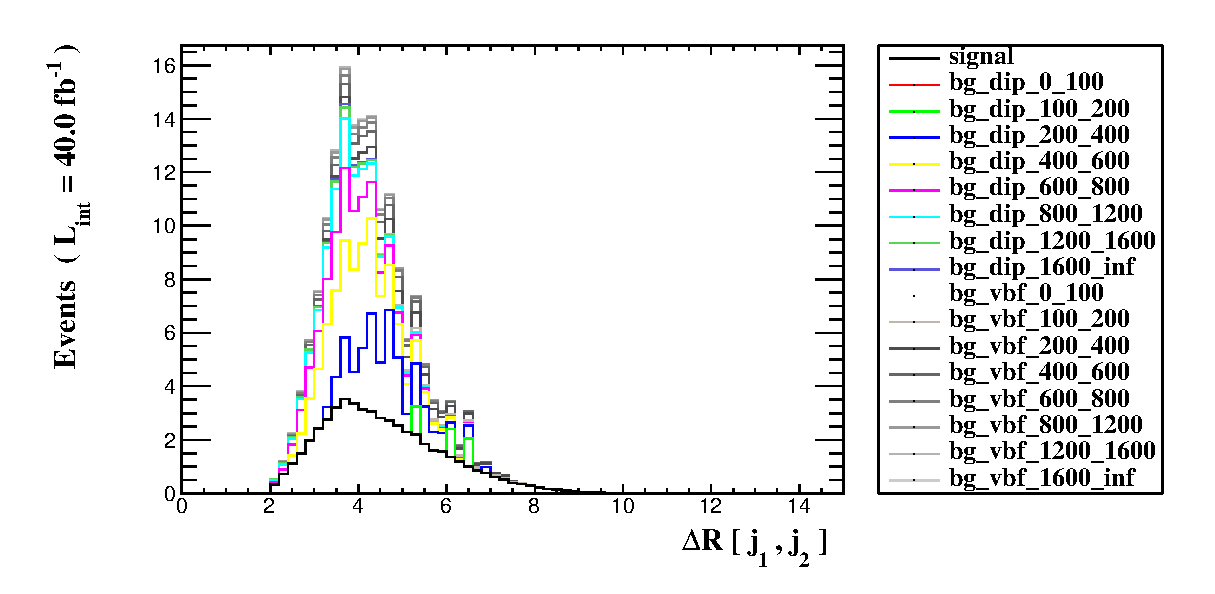
\includegraphics[scale=0.45]{selection_6.eps}\\
\caption{   }
  \end{center}
\end{figure}
      \newpage
\subsection{ Histogram 8}

\textbf{* Plot: M ( jets[1] jets[2] ) }\\
   \begin{table}[H]
  \begin{center}
    \begin{tabular}{|m{23.0mm}|m{23.0mm}|m{18.0mm}|m{19.0mm}|m{19.0mm}|m{19.0mm}|m{19.0mm}|}
      \hline
      {\cellcolor{yellow}         Dataset}& {\cellcolor{yellow}         Integral}& {\cellcolor{yellow}         Entries per event}& {\cellcolor{yellow}         Mean}& {\cellcolor{yellow}         RMS}& {\cellcolor{yellow}         \% underflow}& {\cellcolor{yellow}         \% overflow}\\
      \hline
      {\cellcolor{white}         signal}& {\cellcolor{white}         52.9}& {\cellcolor{white}         1.0}& {\cellcolor{white}         1665.19}& {\cellcolor{white}         783.1}& {\cellcolor{green}         0.0}& {\cellcolor{green}         0.002023}\\
      \hline
      {\cellcolor{white}         bg\_dip\_0\_100}& {\cellcolor{white}         0.0 +/\-- 0.0}& {\cellcolor{white}         0.}& {\cellcolor{white}         0.0}& {\cellcolor{white}         0.0}& {\cellcolor{green}         0.0}& {\cellcolor{green}         0.0}\\
      \hline
      {\cellcolor{white}         bg\_dip\_100\_200}& {\cellcolor{white}         3.16}& {\cellcolor{white}         1.0}& {\cellcolor{white}         1172.68}& {\cellcolor{white}         166.8}& {\cellcolor{green}         0.0}& {\cellcolor{green}         0.0}\\
      \hline
      {\cellcolor{white}         bg\_dip\_200\_400}& {\cellcolor{white}         25.8}& {\cellcolor{white}         1.0}& {\cellcolor{white}         1086.69}& {\cellcolor{white}         339.7}& {\cellcolor{green}         0.0}& {\cellcolor{green}         0.0}\\
      \hline
      {\cellcolor{white}         bg\_dip\_400\_600}& {\cellcolor{white}         34.8}& {\cellcolor{white}         1.0}& {\cellcolor{white}         1108.51}& {\cellcolor{white}         363.5}& {\cellcolor{green}         0.0}& {\cellcolor{green}         0.0}\\
      \hline
      {\cellcolor{white}         bg\_dip\_600\_800}& {\cellcolor{white}         18.8}& {\cellcolor{white}         1.0}& {\cellcolor{white}         1260.28}& {\cellcolor{white}         434.4}& {\cellcolor{green}         0.0}& {\cellcolor{green}         0.0}\\
      \hline
      {\cellcolor{white}         bg\_dip\_800\_1200}& {\cellcolor{white}         11.4}& {\cellcolor{white}         1.0}& {\cellcolor{white}         1581.5}& {\cellcolor{white}         568.2}& {\cellcolor{green}         0.0}& {\cellcolor{green}         0.0}\\
      \hline
      {\cellcolor{white}         bg\_dip\_1200\_1600}& {\cellcolor{white}         1.92}& {\cellcolor{white}         1.0}& {\cellcolor{white}         2160.02}& {\cellcolor{white}         744.2}& {\cellcolor{green}         0.0}& {\cellcolor{green}         0.0}\\
      \hline
      {\cellcolor{white}         bg\_dip\_1600\_inf}& {\cellcolor{white}         0.492}& {\cellcolor{white}         1.0}& {\cellcolor{white}         3060.71}& {\cellcolor{white}         890.4}& {\cellcolor{green}         0.0}& {\cellcolor{green}         0.0}\\
      \hline
      {\cellcolor{white}         bg\_vbf\_0\_100}& {\cellcolor{white}         0.0486}& {\cellcolor{white}         1.0}& {\cellcolor{white}         886.102}& {\cellcolor{white}         84.95}& {\cellcolor{green}         0.0}& {\cellcolor{green}         0.0}\\
      \hline
      {\cellcolor{white}         bg\_vbf\_100\_200}& {\cellcolor{white}         1.16}& {\cellcolor{white}         1.0}& {\cellcolor{white}         1373.99}& {\cellcolor{white}         562.4}& {\cellcolor{green}         0.0}& {\cellcolor{green}         0.0}\\
      \hline
      {\cellcolor{white}         bg\_vbf\_200\_400}& {\cellcolor{white}         6.68}& {\cellcolor{white}         1.0}& {\cellcolor{white}         1609.96}& {\cellcolor{white}         785.9}& {\cellcolor{green}         0.0}& {\cellcolor{green}         0.0}\\
      \hline
      {\cellcolor{white}         bg\_vbf\_400\_600}& {\cellcolor{white}         7.09}& {\cellcolor{white}         1.0}& {\cellcolor{white}         1683.8}& {\cellcolor{white}         828.2}& {\cellcolor{green}         0.0}& {\cellcolor{green}         0.0}\\
      \hline
      {\cellcolor{white}         bg\_vbf\_600\_800}& {\cellcolor{white}         3.66}& {\cellcolor{white}         1.0}& {\cellcolor{white}         1843.6}& {\cellcolor{white}         850.5}& {\cellcolor{green}         0.0}& {\cellcolor{green}         0.0}\\
      \hline
      {\cellcolor{white}         bg\_vbf\_800\_1200}& {\cellcolor{white}         2.15}& {\cellcolor{white}         1.0}& {\cellcolor{white}         2099.49}& {\cellcolor{white}         865.8}& {\cellcolor{green}         0.0}& {\cellcolor{green}         0.0}\\
      \hline
      {\cellcolor{white}         bg\_vbf\_1200\_1600}& {\cellcolor{white}         0.385}& {\cellcolor{white}         1.0}& {\cellcolor{white}         2594.53}& {\cellcolor{white}         883.7}& {\cellcolor{green}         0.0}& {\cellcolor{green}         0.005615}\\
      \hline
      {\cellcolor{white}         bg\_vbf\_1600\_inf}& {\cellcolor{white}         0.0982}& {\cellcolor{white}         1.0}& {\cellcolor{white}         3248.25}& {\cellcolor{white}         956.8}& {\cellcolor{green}         0.0}& {\cellcolor{green}         0.02892}\\
\hline
    \end{tabular}
  \end{center}
\end{table}

\begin{figure}[H]
  \begin{center}
    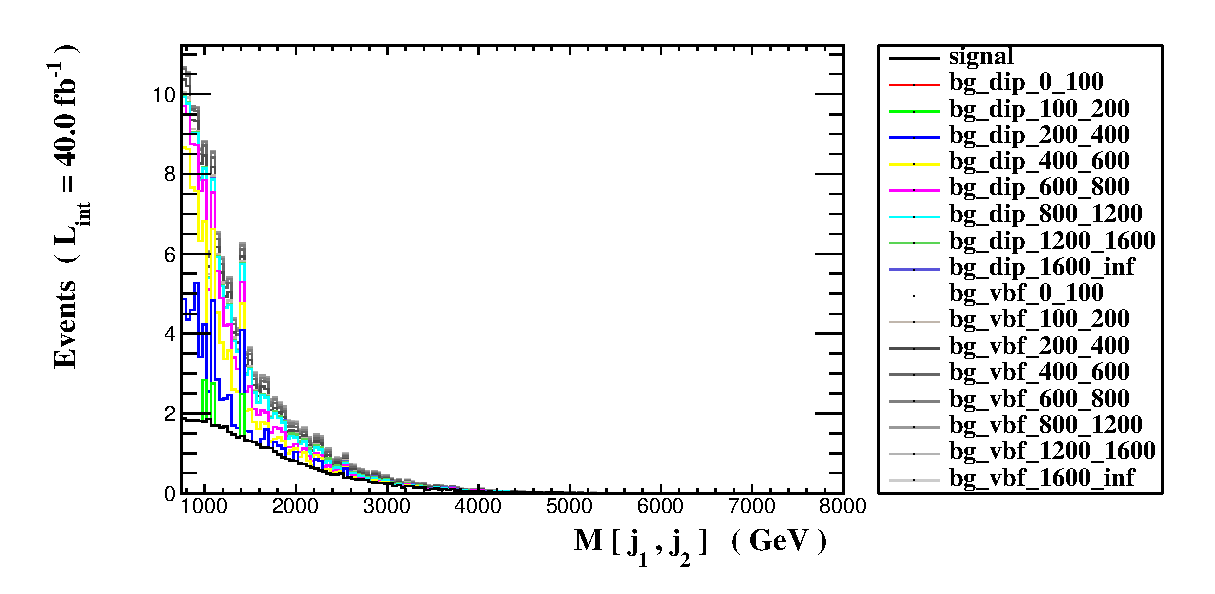
\includegraphics[scale=0.45]{selection_7.eps}\\
\caption{   }
  \end{center}
\end{figure}
      \newpage
\subsection{ Histogram 9}

\textbf{* Plot: sdETA ( jets[1] jets[2] ) }\\
   \begin{table}[H]
  \begin{center}
    \begin{tabular}{|m{23.0mm}|m{23.0mm}|m{18.0mm}|m{19.0mm}|m{19.0mm}|m{19.0mm}|m{19.0mm}|}
      \hline
      {\cellcolor{yellow}         Dataset}& {\cellcolor{yellow}         Integral}& {\cellcolor{yellow}         Entries per event}& {\cellcolor{yellow}         Mean}& {\cellcolor{yellow}         RMS}& {\cellcolor{yellow}         \% underflow}& {\cellcolor{yellow}         \% overflow}\\
      \hline
      {\cellcolor{white}         signal}& {\cellcolor{white}         52.9}& {\cellcolor{white}         1.0}& {\cellcolor{white}         0.000414212}& {\cellcolor{white}         4.407}& {\cellcolor{red}         49.99}& {\cellcolor{red}         0.0}\\
      \hline
      {\cellcolor{white}         bg\_dip\_0\_100}& {\cellcolor{white}         0.0 +/\-- 0.0}& {\cellcolor{white}         0.}& {\cellcolor{white}         0.0}& {\cellcolor{white}         0.0}& {\cellcolor{green}         0.0}& {\cellcolor{green}         0.0}\\
      \hline
      {\cellcolor{white}         bg\_dip\_100\_200}& {\cellcolor{white}         3.16}& {\cellcolor{white}         1.0}& {\cellcolor{white}         1.51032}& {\cellcolor{white}         5.585}& {\cellcolor{red}         33.38}& {\cellcolor{red}         0.0}\\
      \hline
      {\cellcolor{white}         bg\_dip\_200\_400}& {\cellcolor{white}         25.8}& {\cellcolor{white}         1.0}& {\cellcolor{white}         -0.308501}& {\cellcolor{white}         4.231}& {\cellcolor{red}         54.46}& {\cellcolor{red}         0.0}\\
      \hline
      {\cellcolor{white}         bg\_dip\_400\_600}& {\cellcolor{white}         34.8}& {\cellcolor{white}         1.0}& {\cellcolor{white}         0.0970417}& {\cellcolor{white}         3.473}& {\cellcolor{red}         48.45}& {\cellcolor{red}         0.0}\\
      \hline
      {\cellcolor{white}         bg\_dip\_600\_800}& {\cellcolor{white}         18.8}& {\cellcolor{white}         1.0}& {\cellcolor{white}         -0.0870872}& {\cellcolor{white}         3.076}& {\cellcolor{red}         51.5}& {\cellcolor{red}         0.0}\\
      \hline
      {\cellcolor{white}         bg\_dip\_800\_1200}& {\cellcolor{white}         11.4}& {\cellcolor{white}         1.0}& {\cellcolor{white}         0.0393952}& {\cellcolor{white}         2.891}& {\cellcolor{red}         49.24}& {\cellcolor{red}         0.0}\\
      \hline
      {\cellcolor{white}         bg\_dip\_1200\_1600}& {\cellcolor{white}         1.92}& {\cellcolor{white}         1.0}& {\cellcolor{white}         -0.0394215}& {\cellcolor{white}         2.694}& {\cellcolor{red}         50.67}& {\cellcolor{red}         0.0}\\
      \hline
      {\cellcolor{white}         bg\_dip\_1600\_inf}& {\cellcolor{white}         0.492}& {\cellcolor{white}         1.0}& {\cellcolor{white}         0.082972}& {\cellcolor{white}         2.48}& {\cellcolor{red}         48.4}& {\cellcolor{red}         0.0}\\
      \hline
      {\cellcolor{white}         bg\_vbf\_0\_100}& {\cellcolor{white}         0.0486}& {\cellcolor{white}         1.0}& {\cellcolor{white}         -0.174236}& {\cellcolor{white}         6.403}& {\cellcolor{red}         50.0}& {\cellcolor{red}         0.0}\\
      \hline
      {\cellcolor{white}         bg\_vbf\_100\_200}& {\cellcolor{white}         1.16}& {\cellcolor{white}         1.0}& {\cellcolor{white}         0.457753}& {\cellcolor{white}         5.752}& {\cellcolor{red}         46.55}& {\cellcolor{red}         0.0}\\
      \hline
      {\cellcolor{white}         bg\_vbf\_200\_400}& {\cellcolor{white}         6.68}& {\cellcolor{white}         1.0}& {\cellcolor{white}         -0.0210876}& {\cellcolor{white}         4.873}& {\cellcolor{red}         50.04}& {\cellcolor{red}         0.0}\\
      \hline
      {\cellcolor{white}         bg\_vbf\_400\_600}& {\cellcolor{white}         7.09}& {\cellcolor{white}         1.0}& {\cellcolor{white}         -0.0608118}& {\cellcolor{white}         4.106}& {\cellcolor{red}         50.68}& {\cellcolor{red}         0.0}\\
      \hline
      {\cellcolor{white}         bg\_vbf\_600\_800}& {\cellcolor{white}         3.66}& {\cellcolor{white}         1.0}& {\cellcolor{white}         -0.00763357}& {\cellcolor{white}         3.637}& {\cellcolor{red}         50.18}& {\cellcolor{red}         0.0}\\
      \hline
      {\cellcolor{white}         bg\_vbf\_800\_1200}& {\cellcolor{white}         2.15}& {\cellcolor{white}         1.0}& {\cellcolor{white}         -0.0731017}& {\cellcolor{white}         3.293}& {\cellcolor{red}         51.18}& {\cellcolor{red}         0.0}\\
      \hline
      {\cellcolor{white}         bg\_vbf\_1200\_1600}& {\cellcolor{white}         0.385}& {\cellcolor{white}         1.0}& {\cellcolor{white}         -0.0409604}& {\cellcolor{white}         2.969}& {\cellcolor{red}         50.52}& {\cellcolor{red}         0.0}\\
      \hline
      {\cellcolor{white}         bg\_vbf\_1600\_inf}& {\cellcolor{white}         0.0982}& {\cellcolor{white}         1.0}& {\cellcolor{white}         0.0465608}& {\cellcolor{white}         2.701}& {\cellcolor{red}         49.38}& {\cellcolor{red}         0.0}\\
\hline
    \end{tabular}
  \end{center}
\end{table}

\begin{figure}[H]
  \begin{center}
    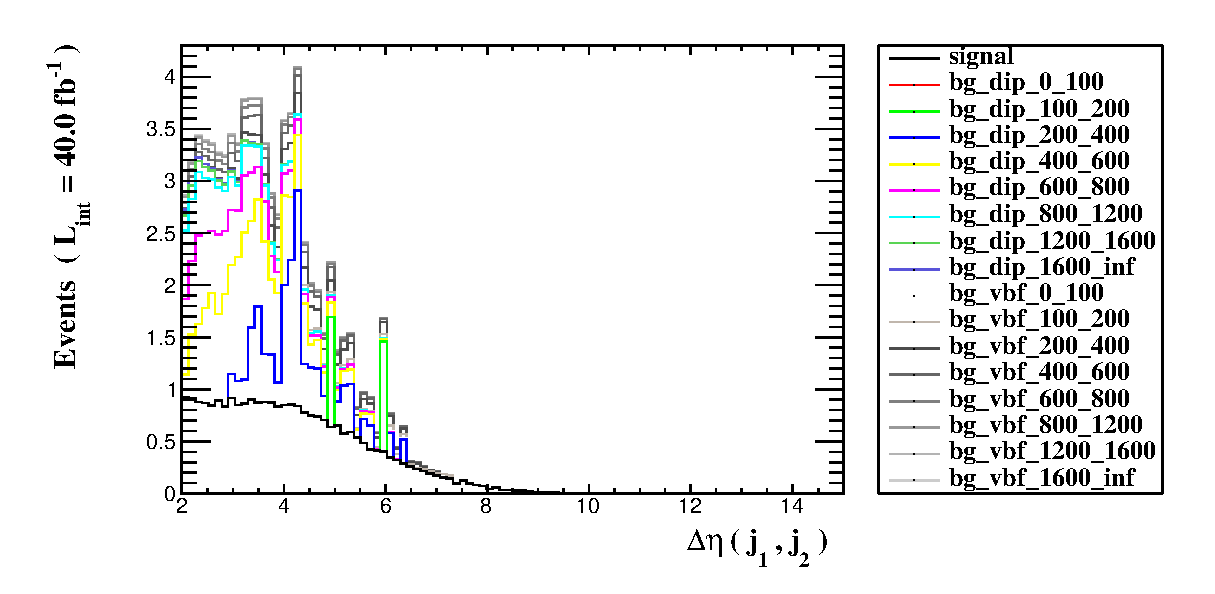
\includegraphics[scale=0.45]{selection_8.eps}\\
\caption{   }
  \end{center}
\end{figure}
      \newpage
\subsection{ Histogram 10}

\textbf{* Plot: M ( a[1] a[2] ) }\\
   \begin{table}[H]
  \begin{center}
    \begin{tabular}{|m{23.0mm}|m{23.0mm}|m{18.0mm}|m{19.0mm}|m{19.0mm}|m{19.0mm}|m{19.0mm}|}
      \hline
      {\cellcolor{yellow}         Dataset}& {\cellcolor{yellow}         Integral}& {\cellcolor{yellow}         Entries per event}& {\cellcolor{yellow}         Mean}& {\cellcolor{yellow}         RMS}& {\cellcolor{yellow}         \% underflow}& {\cellcolor{yellow}         \% overflow}\\
      \hline
      {\cellcolor{white}         signal}& {\cellcolor{white}         52.9}& {\cellcolor{white}         1.0}& {\cellcolor{white}         1430.57}& {\cellcolor{white}         799.7}& {\cellcolor{green}         0.0}& {\cellcolor{green}         1.182}\\
      \hline
      {\cellcolor{white}         bg\_dip\_0\_100}& {\cellcolor{white}         0.0 +/\-- 0.0}& {\cellcolor{white}         0.}& {\cellcolor{white}         0.0}& {\cellcolor{white}         0.0}& {\cellcolor{green}         0.0}& {\cellcolor{green}         0.0}\\
      \hline
      {\cellcolor{white}         bg\_dip\_100\_200}& {\cellcolor{white}         3.16}& {\cellcolor{white}         1.0}& {\cellcolor{white}         674.287}& {\cellcolor{white}         36.08}& {\cellcolor{green}         0.0}& {\cellcolor{green}         0.0}\\
      \hline
      {\cellcolor{white}         bg\_dip\_200\_400}& {\cellcolor{white}         25.8}& {\cellcolor{white}         1.0}& {\cellcolor{white}         806.444}& {\cellcolor{white}         369.4}& {\cellcolor{green}         0.0}& {\cellcolor{green}         0.0}\\
      \hline
      {\cellcolor{white}         bg\_dip\_400\_600}& {\cellcolor{white}         34.8}& {\cellcolor{white}         1.0}& {\cellcolor{white}         756.124}& {\cellcolor{white}         297.2}& {\cellcolor{green}         0.0}& {\cellcolor{green}         0.0}\\
      \hline
      {\cellcolor{white}         bg\_dip\_600\_800}& {\cellcolor{white}         18.8}& {\cellcolor{white}         1.0}& {\cellcolor{white}         781.031}& {\cellcolor{white}         322.1}& {\cellcolor{green}         0.0}& {\cellcolor{green}         0.0}\\
      \hline
      {\cellcolor{white}         bg\_dip\_800\_1200}& {\cellcolor{white}         11.4}& {\cellcolor{white}         1.0}& {\cellcolor{white}         814.453}& {\cellcolor{white}         348.2}& {\cellcolor{green}         0.0}& {\cellcolor{green}         0.0}\\
      \hline
      {\cellcolor{white}         bg\_dip\_1200\_1600}& {\cellcolor{white}         1.92}& {\cellcolor{white}         1.0}& {\cellcolor{white}         844.472}& {\cellcolor{white}         365.4}& {\cellcolor{green}         0.0}& {\cellcolor{green}         0.0}\\
      \hline
      {\cellcolor{white}         bg\_dip\_1600\_inf}& {\cellcolor{white}         0.492}& {\cellcolor{white}         1.0}& {\cellcolor{white}         872.363}& {\cellcolor{white}         403.7}& {\cellcolor{green}         0.0}& {\cellcolor{green}         0.0}\\
      \hline
      {\cellcolor{white}         bg\_vbf\_0\_100}& {\cellcolor{white}         0.0486}& {\cellcolor{white}         1.0}& {\cellcolor{white}         999.408}& {\cellcolor{white}         375.3}& {\cellcolor{green}         0.0}& {\cellcolor{green}         0.0}\\
      \hline
      {\cellcolor{white}         bg\_vbf\_100\_200}& {\cellcolor{white}         1.16}& {\cellcolor{white}         1.0}& {\cellcolor{white}         847.835}& {\cellcolor{white}         279.9}& {\cellcolor{green}         0.0}& {\cellcolor{green}         0.0}\\
      \hline
      {\cellcolor{white}         bg\_vbf\_200\_400}& {\cellcolor{white}         6.68}& {\cellcolor{white}         1.0}& {\cellcolor{white}         801.713}& {\cellcolor{white}         329.2}& {\cellcolor{green}         0.0}& {\cellcolor{green}         0.0}\\
      \hline
      {\cellcolor{white}         bg\_vbf\_400\_600}& {\cellcolor{white}         7.09}& {\cellcolor{white}         1.0}& {\cellcolor{white}         750.135}& {\cellcolor{white}         282.4}& {\cellcolor{green}         0.0}& {\cellcolor{green}         0.0}\\
      \hline
      {\cellcolor{white}         bg\_vbf\_600\_800}& {\cellcolor{white}         3.66}& {\cellcolor{white}         1.0}& {\cellcolor{white}         761.9}& {\cellcolor{white}         286.2}& {\cellcolor{green}         0.0}& {\cellcolor{green}         0.0}\\
      \hline
      {\cellcolor{white}         bg\_vbf\_800\_1200}& {\cellcolor{white}         2.15}& {\cellcolor{white}         1.0}& {\cellcolor{white}         780.346}& {\cellcolor{white}         299.0}& {\cellcolor{green}         0.0}& {\cellcolor{green}         0.0}\\
      \hline
      {\cellcolor{white}         bg\_vbf\_1200\_1600}& {\cellcolor{white}         0.385}& {\cellcolor{white}         1.0}& {\cellcolor{white}         798.746}& {\cellcolor{white}         322.8}& {\cellcolor{green}         0.0}& {\cellcolor{green}         0.02242}\\
      \hline
      {\cellcolor{white}         bg\_vbf\_1600\_inf}& {\cellcolor{white}         0.0982}& {\cellcolor{white}         1.0}& {\cellcolor{white}         824.802}& {\cellcolor{white}         350.7}& {\cellcolor{green}         0.0}& {\cellcolor{green}         0.02892}\\
\hline
    \end{tabular}
  \end{center}
\end{table}

\begin{figure}[H]
  \begin{center}
    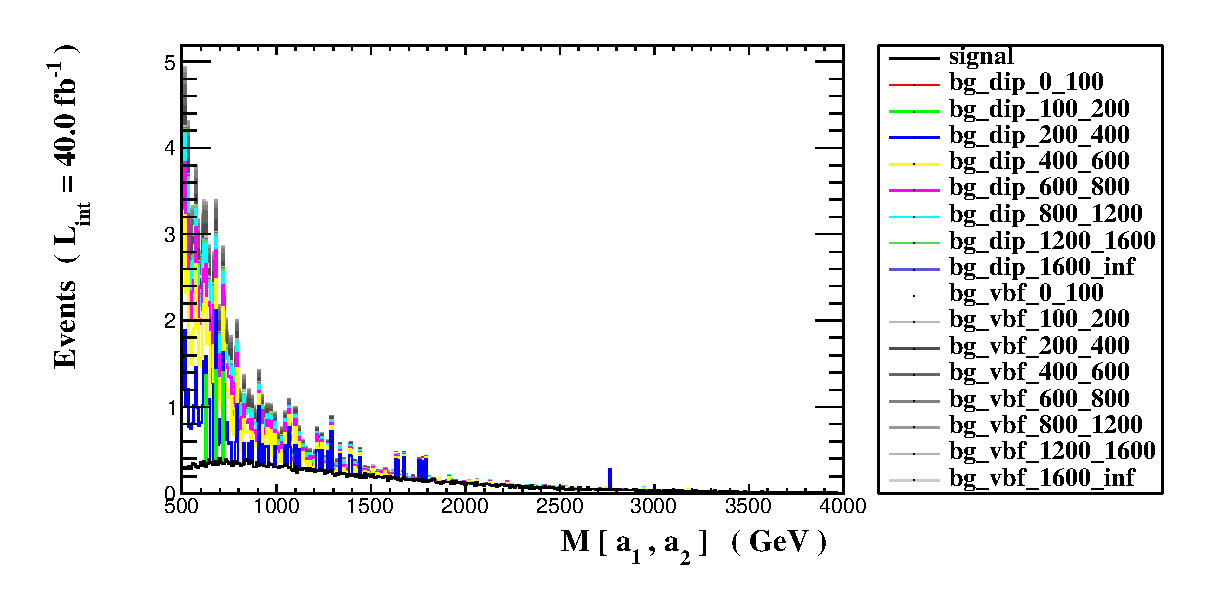
\includegraphics[scale=0.45]{selection_9.eps}\\
\caption{   }
  \end{center}
\end{figure}
      \newpage
\subsection{ Histogram 11}

\textbf{* Plot: PT ( a[1] ) }\\
   \begin{table}[H]
  \begin{center}
    \begin{tabular}{|m{23.0mm}|m{23.0mm}|m{18.0mm}|m{19.0mm}|m{19.0mm}|m{19.0mm}|m{19.0mm}|}
      \hline
      {\cellcolor{yellow}         Dataset}& {\cellcolor{yellow}         Integral}& {\cellcolor{yellow}         Entries per event}& {\cellcolor{yellow}         Mean}& {\cellcolor{yellow}         RMS}& {\cellcolor{yellow}         \% underflow}& {\cellcolor{yellow}         \% overflow}\\
      \hline
      {\cellcolor{white}         signal}& {\cellcolor{white}         52.9}& {\cellcolor{white}         1.0}& {\cellcolor{white}         775.56}& {\cellcolor{white}         380.5}& {\cellcolor{green}         0.0}& {\cellcolor{green}         1.059}\\
      \hline
      {\cellcolor{white}         bg\_dip\_0\_100}& {\cellcolor{white}         0.0 +/\-- 0.0}& {\cellcolor{white}         0.}& {\cellcolor{white}         0.0}& {\cellcolor{white}         0.0}& {\cellcolor{green}         0.0}& {\cellcolor{green}         0.0}\\
      \hline
      {\cellcolor{white}         bg\_dip\_100\_200}& {\cellcolor{white}         3.16}& {\cellcolor{white}         1.0}& {\cellcolor{white}         327.174}& {\cellcolor{white}         7.434}& {\cellcolor{green}         0.0}& {\cellcolor{green}         0.0}\\
      \hline
      {\cellcolor{white}         bg\_dip\_200\_400}& {\cellcolor{white}         25.8}& {\cellcolor{white}         1.0}& {\cellcolor{white}         400.151}& {\cellcolor{white}         82.89}& {\cellcolor{green}         0.0}& {\cellcolor{green}         0.0}\\
      \hline
      {\cellcolor{white}         bg\_dip\_400\_600}& {\cellcolor{white}         34.8}& {\cellcolor{white}         1.0}& {\cellcolor{white}         445.165}& {\cellcolor{white}         113.4}& {\cellcolor{green}         0.0}& {\cellcolor{green}         0.0}\\
      \hline
      {\cellcolor{white}         bg\_dip\_600\_800}& {\cellcolor{white}         18.8}& {\cellcolor{white}         1.0}& {\cellcolor{white}         529.399}& {\cellcolor{white}         160.6}& {\cellcolor{green}         0.0}& {\cellcolor{green}         0.0}\\
      \hline
      {\cellcolor{white}         bg\_dip\_800\_1200}& {\cellcolor{white}         11.4}& {\cellcolor{white}         1.0}& {\cellcolor{white}         638.285}& {\cellcolor{white}         244.3}& {\cellcolor{green}         0.0}& {\cellcolor{green}         0.02474}\\
      \hline
      {\cellcolor{white}         bg\_dip\_1200\_1600}& {\cellcolor{white}         1.92}& {\cellcolor{white}         1.0}& {\cellcolor{white}         750.786}& {\cellcolor{white}         377.2}& {\cellcolor{green}         0.0}& {\cellcolor{green}         0.0}\\
      \hline
      {\cellcolor{white}         bg\_dip\_1600\_inf}& {\cellcolor{white}         0.492}& {\cellcolor{white}         1.0}& {\cellcolor{white}         746.417}& {\cellcolor{white}         471.4}& {\cellcolor{green}         0.0}& {\cellcolor{green}         1.725}\\
      \hline
      {\cellcolor{white}         bg\_vbf\_0\_100}& {\cellcolor{white}         0.0486}& {\cellcolor{white}         1.0}& {\cellcolor{white}         379.899}& {\cellcolor{white}         64.59}& {\cellcolor{green}         0.0}& {\cellcolor{green}         0.0}\\
      \hline
      {\cellcolor{white}         bg\_vbf\_100\_200}& {\cellcolor{white}         1.16}& {\cellcolor{white}         1.0}& {\cellcolor{white}         373.902}& {\cellcolor{white}         77.67}& {\cellcolor{green}         0.0}& {\cellcolor{green}         0.0}\\
      \hline
      {\cellcolor{white}         bg\_vbf\_200\_400}& {\cellcolor{white}         6.68}& {\cellcolor{white}         1.0}& {\cellcolor{white}         392.202}& {\cellcolor{white}         92.25}& {\cellcolor{green}         0.0}& {\cellcolor{green}         0.0}\\
      \hline
      {\cellcolor{white}         bg\_vbf\_400\_600}& {\cellcolor{white}         7.09}& {\cellcolor{white}         1.0}& {\cellcolor{white}         436.628}& {\cellcolor{white}         112.8}& {\cellcolor{green}         0.0}& {\cellcolor{green}         0.0}\\
      \hline
      {\cellcolor{white}         bg\_vbf\_600\_800}& {\cellcolor{white}         3.66}& {\cellcolor{white}         1.0}& {\cellcolor{white}         508.867}& {\cellcolor{white}         149.0}& {\cellcolor{green}         0.0}& {\cellcolor{green}         0.0}\\
      \hline
      {\cellcolor{white}         bg\_vbf\_800\_1200}& {\cellcolor{white}         2.15}& {\cellcolor{white}         1.0}& {\cellcolor{white}         620.887}& {\cellcolor{white}         223.3}& {\cellcolor{green}         0.0}& {\cellcolor{green}         0.0}\\
      \hline
      {\cellcolor{white}         bg\_vbf\_1200\_1600}& {\cellcolor{white}         0.385}& {\cellcolor{white}         1.0}& {\cellcolor{white}         762.723}& {\cellcolor{white}         338.6}& {\cellcolor{green}         0.0}& {\cellcolor{green}         0.028}\\
      \hline
      {\cellcolor{white}         bg\_vbf\_1600\_inf}& {\cellcolor{white}         0.0982}& {\cellcolor{white}         1.0}& {\cellcolor{white}         874.736}& {\cellcolor{white}         484.8}& {\cellcolor{green}         0.0}& {\cellcolor{green}         1.73}\\
\hline
    \end{tabular}
  \end{center}
\end{table}

\begin{figure}[H]
  \begin{center}
    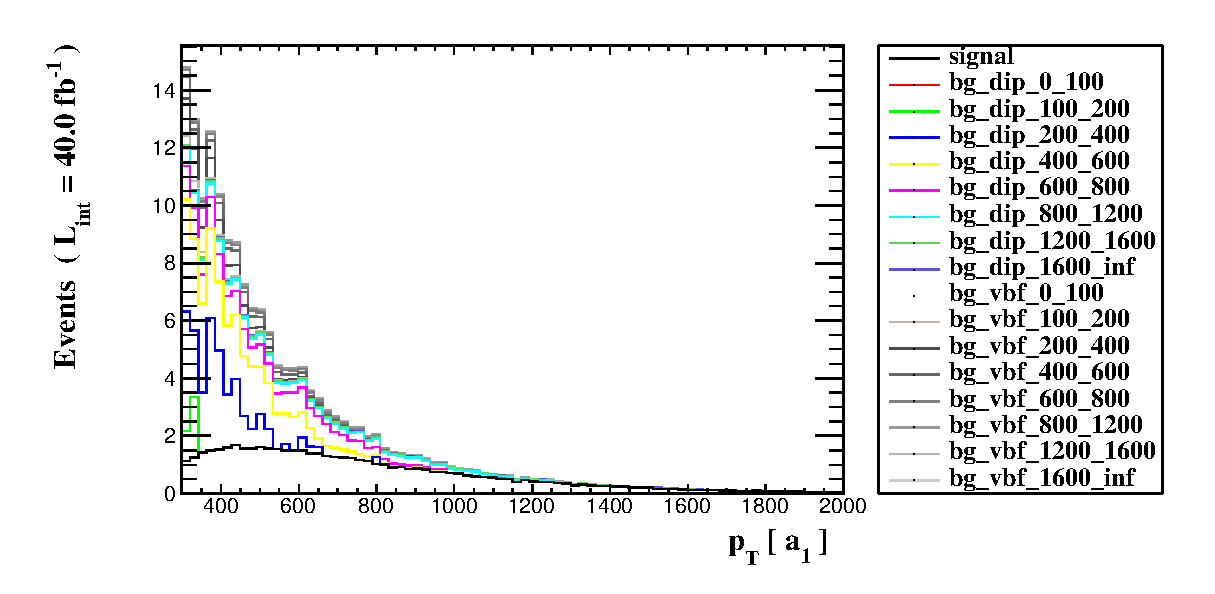
\includegraphics[scale=0.45]{selection_10.eps}\\
\caption{   }
  \end{center}
\end{figure}
      \newpage
\subsection{ Histogram 12}

\textbf{* Plot: PT ( a[2] ) }\\
   \begin{table}[H]
  \begin{center}
    \begin{tabular}{|m{23.0mm}|m{23.0mm}|m{18.0mm}|m{19.0mm}|m{19.0mm}|m{19.0mm}|m{19.0mm}|}
      \hline
      {\cellcolor{yellow}         Dataset}& {\cellcolor{yellow}         Integral}& {\cellcolor{yellow}         Entries per event}& {\cellcolor{yellow}         Mean}& {\cellcolor{yellow}         RMS}& {\cellcolor{yellow}         \% underflow}& {\cellcolor{yellow}         \% overflow}\\
      \hline
      {\cellcolor{white}         signal}& {\cellcolor{white}         52.9}& {\cellcolor{white}         1.0}& {\cellcolor{white}         507.74}& {\cellcolor{white}         344.5}& {\cellcolor{green}         0.0}& {\cellcolor{green}         0.3779}\\
      \hline
      {\cellcolor{white}         bg\_dip\_0\_100}& {\cellcolor{white}         0.0 +/\-- 0.0}& {\cellcolor{white}         0.}& {\cellcolor{white}         0.0}& {\cellcolor{white}         0.0}& {\cellcolor{green}         0.0}& {\cellcolor{green}         0.0}\\
      \hline
      {\cellcolor{white}         bg\_dip\_100\_200}& {\cellcolor{white}         3.16}& {\cellcolor{white}         1.0}& {\cellcolor{white}         253.391}& {\cellcolor{white}         44.39}& {\cellcolor{green}         0.0}& {\cellcolor{green}         0.0}\\
      \hline
      {\cellcolor{white}         bg\_dip\_200\_400}& {\cellcolor{white}         25.8}& {\cellcolor{white}         1.0}& {\cellcolor{white}         191.937}& {\cellcolor{white}         101.6}& {\cellcolor{green}         0.0}& {\cellcolor{green}         0.0}\\
      \hline
      {\cellcolor{white}         bg\_dip\_400\_600}& {\cellcolor{white}         34.8}& {\cellcolor{white}         1.0}& {\cellcolor{white}         143.019}& {\cellcolor{white}         101.1}& {\cellcolor{green}         0.0}& {\cellcolor{green}         0.0}\\
      \hline
      {\cellcolor{white}         bg\_dip\_600\_800}& {\cellcolor{white}         18.8}& {\cellcolor{white}         1.0}& {\cellcolor{white}         139.123}& {\cellcolor{white}         105.0}& {\cellcolor{green}         0.0}& {\cellcolor{green}         0.0}\\
      \hline
      {\cellcolor{white}         bg\_dip\_800\_1200}& {\cellcolor{white}         11.4}& {\cellcolor{white}         1.0}& {\cellcolor{white}         138.571}& {\cellcolor{white}         114.8}& {\cellcolor{green}         0.0}& {\cellcolor{green}         0.0}\\
      \hline
      {\cellcolor{white}         bg\_dip\_1200\_1600}& {\cellcolor{white}         1.92}& {\cellcolor{white}         1.0}& {\cellcolor{white}         131.66}& {\cellcolor{white}         116.5}& {\cellcolor{green}         0.0}& {\cellcolor{green}         0.0}\\
      \hline
      {\cellcolor{white}         bg\_dip\_1600\_inf}& {\cellcolor{white}         0.492}& {\cellcolor{white}         1.0}& {\cellcolor{white}         138.93}& {\cellcolor{white}         127.7}& {\cellcolor{green}         0.0}& {\cellcolor{green}         0.0}\\
      \hline
      {\cellcolor{white}         bg\_vbf\_0\_100}& {\cellcolor{white}         0.0486}& {\cellcolor{white}         1.0}& {\cellcolor{white}         359.837}& {\cellcolor{white}         74.21}& {\cellcolor{green}         0.0}& {\cellcolor{green}         0.0}\\
      \hline
      {\cellcolor{white}         bg\_vbf\_100\_200}& {\cellcolor{white}         1.16}& {\cellcolor{white}         1.0}& {\cellcolor{white}         285.217}& {\cellcolor{white}         94.57}& {\cellcolor{green}         0.0}& {\cellcolor{green}         0.0}\\
      \hline
      {\cellcolor{white}         bg\_vbf\_200\_400}& {\cellcolor{white}         6.68}& {\cellcolor{white}         1.0}& {\cellcolor{white}         209.279}& {\cellcolor{white}         119.1}& {\cellcolor{green}         0.0}& {\cellcolor{green}         0.0}\\
      \hline
      {\cellcolor{white}         bg\_vbf\_400\_600}& {\cellcolor{white}         7.09}& {\cellcolor{white}         1.0}& {\cellcolor{white}         164.173}& {\cellcolor{white}         118.0}& {\cellcolor{green}         0.0}& {\cellcolor{green}         0.0}\\
      \hline
      {\cellcolor{white}         bg\_vbf\_600\_800}& {\cellcolor{white}         3.66}& {\cellcolor{white}         1.0}& {\cellcolor{white}         162.598}& {\cellcolor{white}         113.4}& {\cellcolor{green}         0.0}& {\cellcolor{green}         0.0}\\
      \hline
      {\cellcolor{white}         bg\_vbf\_800\_1200}& {\cellcolor{white}         2.15}& {\cellcolor{white}         1.0}& {\cellcolor{white}         169.681}& {\cellcolor{white}         124.3}& {\cellcolor{green}         0.0}& {\cellcolor{green}         0.0}\\
      \hline
      {\cellcolor{white}         bg\_vbf\_1200\_1600}& {\cellcolor{white}         0.385}& {\cellcolor{white}         1.0}& {\cellcolor{white}         175.082}& {\cellcolor{white}         135.1}& {\cellcolor{green}         0.0}& {\cellcolor{green}         0.0}\\
      \hline
      {\cellcolor{white}         bg\_vbf\_1600\_inf}& {\cellcolor{white}         0.0982}& {\cellcolor{white}         1.0}& {\cellcolor{white}         183.775}& {\cellcolor{white}         152.5}& {\cellcolor{green}         0.0}& {\cellcolor{green}         0.0}\\
\hline
    \end{tabular}
  \end{center}
\end{table}

\begin{figure}[H]
  \begin{center}
    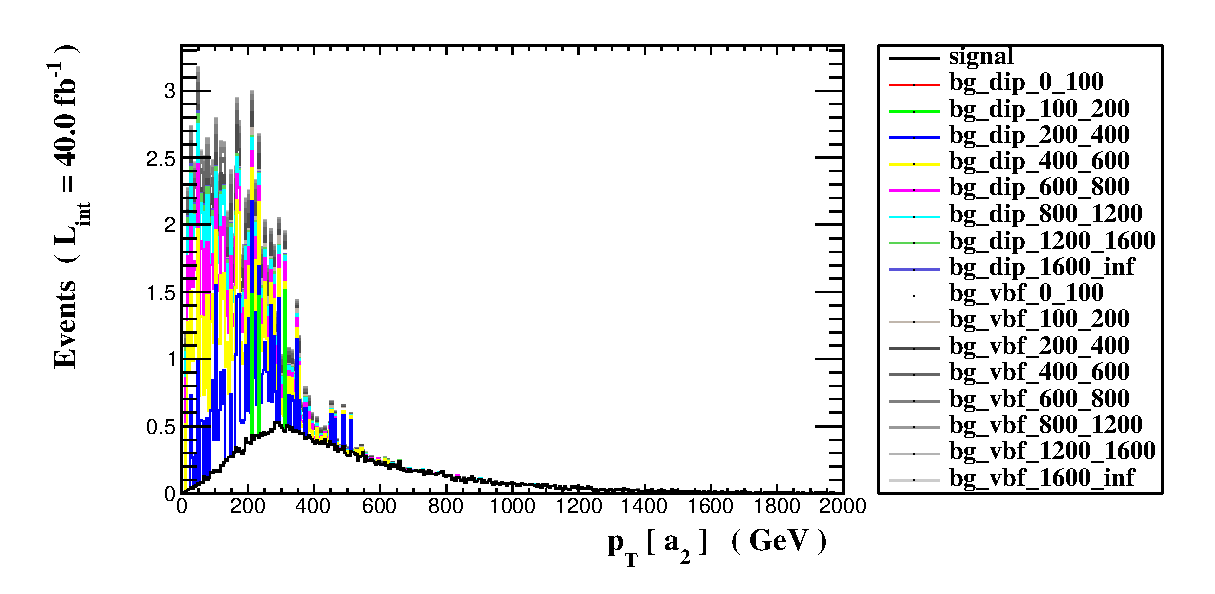
\includegraphics[scale=0.45]{selection_11.eps}\\
\caption{   }
  \end{center}
\end{figure}
      \newpage
\subsection{ Histogram 13}

\textbf{* Plot: THT}\\
   \begin{table}[H]
  \begin{center}
    \begin{tabular}{|m{23.0mm}|m{23.0mm}|m{18.0mm}|m{19.0mm}|m{19.0mm}|m{19.0mm}|m{19.0mm}|}
      \hline
      {\cellcolor{yellow}         Dataset}& {\cellcolor{yellow}         Integral}& {\cellcolor{yellow}         Entries per event}& {\cellcolor{yellow}         Mean}& {\cellcolor{yellow}         RMS}& {\cellcolor{yellow}         \% underflow}& {\cellcolor{yellow}         \% overflow}\\
      \hline
      {\cellcolor{white}         signal}& {\cellcolor{white}         52.9}& {\cellcolor{white}         1.0}& {\cellcolor{white}         587.037}& {\cellcolor{white}         392.4}& {\cellcolor{green}         0.0}& {\cellcolor{green}         0.0}\\
      \hline
      {\cellcolor{white}         bg\_dip\_0\_100}& {\cellcolor{white}         0.0 +/\-- 0.0}& {\cellcolor{white}         0.}& {\cellcolor{white}         0.0}& {\cellcolor{white}         0.0}& {\cellcolor{green}         0.0}& {\cellcolor{green}         0.0}\\
      \hline
      {\cellcolor{white}         bg\_dip\_100\_200}& {\cellcolor{white}         3.16}& {\cellcolor{white}         1.0}& {\cellcolor{white}         148.168}& {\cellcolor{white}         37.58}& {\cellcolor{green}         0.0}& {\cellcolor{green}         0.0}\\
      \hline
      {\cellcolor{white}         bg\_dip\_200\_400}& {\cellcolor{white}         25.8}& {\cellcolor{white}         1.0}& {\cellcolor{white}         322.57}& {\cellcolor{white}         51.94}& {\cellcolor{green}         0.0}& {\cellcolor{green}         0.0}\\
      \hline
      {\cellcolor{white}         bg\_dip\_400\_600}& {\cellcolor{white}         34.8}& {\cellcolor{white}         1.0}& {\cellcolor{white}         497.625}& {\cellcolor{white}         57.16}& {\cellcolor{green}         0.0}& {\cellcolor{green}         0.0}\\
      \hline
      {\cellcolor{white}         bg\_dip\_600\_800}& {\cellcolor{white}         18.8}& {\cellcolor{white}         1.0}& {\cellcolor{white}         687.176}& {\cellcolor{white}         55.95}& {\cellcolor{green}         0.0}& {\cellcolor{green}         0.0}\\
      \hline
      {\cellcolor{white}         bg\_dip\_800\_1200}& {\cellcolor{white}         11.4}& {\cellcolor{white}         1.0}& {\cellcolor{white}         940.982}& {\cellcolor{white}         106.9}& {\cellcolor{green}         0.0}& {\cellcolor{green}         0.0}\\
      \hline
      {\cellcolor{white}         bg\_dip\_1200\_1600}& {\cellcolor{white}         1.92}& {\cellcolor{white}         1.0}& {\cellcolor{white}         1340.97}& {\cellcolor{white}         107.2}& {\cellcolor{green}         0.0}& {\cellcolor{green}         0.0}\\
      \hline
      {\cellcolor{white}         bg\_dip\_1600\_inf}& {\cellcolor{white}         0.492}& {\cellcolor{white}         1.0}& {\cellcolor{white}         1877.37}& {\cellcolor{white}         276.5}& {\cellcolor{green}         0.0}& {\cellcolor{green}         0.0}\\
      \hline
      {\cellcolor{white}         bg\_vbf\_0\_100}& {\cellcolor{white}         0.0486}& {\cellcolor{white}         1.0}& {\cellcolor{white}         74.6978}& {\cellcolor{white}         15.53}& {\cellcolor{green}         0.0}& {\cellcolor{green}         0.0}\\
      \hline
      {\cellcolor{white}         bg\_vbf\_100\_200}& {\cellcolor{white}         1.16}& {\cellcolor{white}         1.0}& {\cellcolor{white}         163.344}& {\cellcolor{white}         25.73}& {\cellcolor{green}         0.0}& {\cellcolor{green}         0.0}\\
      \hline
      {\cellcolor{white}         bg\_vbf\_200\_400}& {\cellcolor{white}         6.68}& {\cellcolor{white}         1.0}& {\cellcolor{white}         310.201}& {\cellcolor{white}         55.23}& {\cellcolor{green}         0.0}& {\cellcolor{green}         0.0}\\
      \hline
      {\cellcolor{white}         bg\_vbf\_400\_600}& {\cellcolor{white}         7.09}& {\cellcolor{white}         1.0}& {\cellcolor{white}         491.892}& {\cellcolor{white}         56.3}& {\cellcolor{green}         0.0}& {\cellcolor{green}         0.0}\\
      \hline
      {\cellcolor{white}         bg\_vbf\_600\_800}& {\cellcolor{white}         3.66}& {\cellcolor{white}         1.0}& {\cellcolor{white}         686.63}& {\cellcolor{white}         56.67}& {\cellcolor{green}         0.0}& {\cellcolor{green}         0.0}\\
      \hline
      {\cellcolor{white}         bg\_vbf\_800\_1200}& {\cellcolor{white}         2.15}& {\cellcolor{white}         1.0}& {\cellcolor{white}         943.126}& {\cellcolor{white}         106.9}& {\cellcolor{green}         0.0}& {\cellcolor{green}         0.0}\\
      \hline
      {\cellcolor{white}         bg\_vbf\_1200\_1600}& {\cellcolor{white}         0.385}& {\cellcolor{white}         1.0}& {\cellcolor{white}         1347.37}& {\cellcolor{white}         108.8}& {\cellcolor{green}         0.0}& {\cellcolor{green}         0.0}\\
      \hline
      {\cellcolor{white}         bg\_vbf\_1600\_inf}& {\cellcolor{white}         0.0982}& {\cellcolor{white}         1.0}& {\cellcolor{white}         1860.8}& {\cellcolor{white}         269.2}& {\cellcolor{green}         0.0}& {\cellcolor{green}         0.02892}\\
\hline
    \end{tabular}
  \end{center}
\end{table}

\begin{figure}[H]
  \begin{center}
    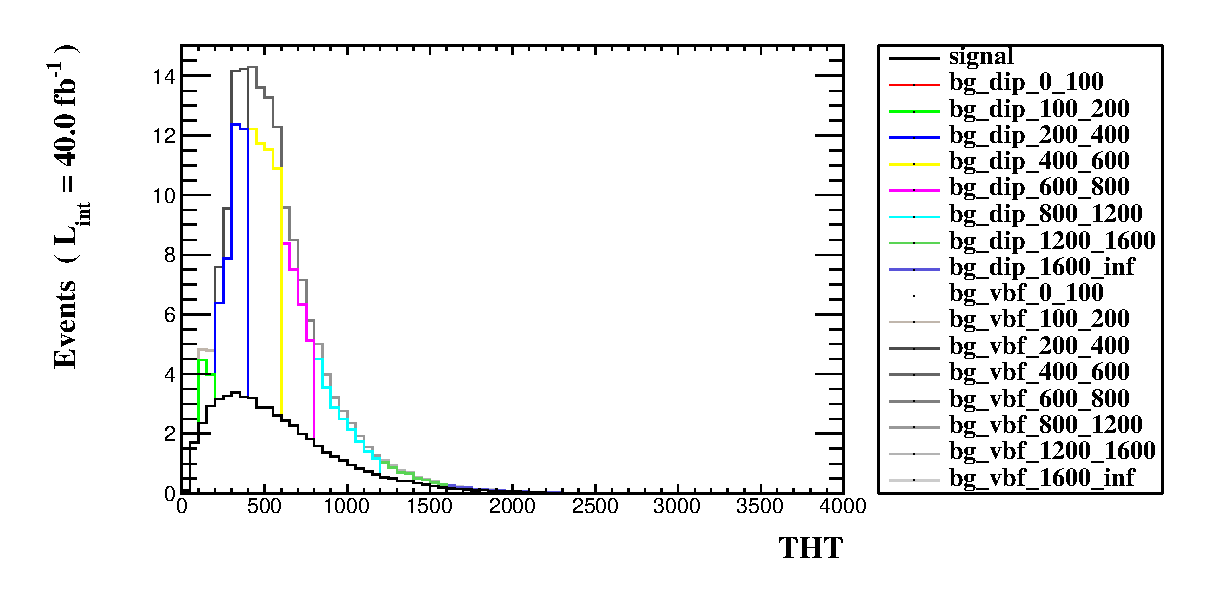
\includegraphics[scale=0.45]{selection_12.eps}\\
\caption{   }
  \end{center}
\end{figure}
      \newpage
\subsection{ Histogram 14}

\textbf{* Plot: MET}\\
   \begin{table}[H]
  \begin{center}
    \begin{tabular}{|m{23.0mm}|m{23.0mm}|m{18.0mm}|m{19.0mm}|m{19.0mm}|m{19.0mm}|m{19.0mm}|}
      \hline
      {\cellcolor{yellow}         Dataset}& {\cellcolor{yellow}         Integral}& {\cellcolor{yellow}         Entries per event}& {\cellcolor{yellow}         Mean}& {\cellcolor{yellow}         RMS}& {\cellcolor{yellow}         \% underflow}& {\cellcolor{yellow}         \% overflow}\\
      \hline
      {\cellcolor{white}         signal}& {\cellcolor{white}         52.9}& {\cellcolor{white}         1.0}& {\cellcolor{white}         1.05124e-08}& {\cellcolor{white}         1.342e-08}& {\cellcolor{green}         0.0}& {\cellcolor{green}         0.0}\\
      \hline
      {\cellcolor{white}         bg\_dip\_0\_100}& {\cellcolor{white}         0.0 +/\-- 0.0}& {\cellcolor{white}         0.}& {\cellcolor{white}         0.0}& {\cellcolor{white}         0.0}& {\cellcolor{green}         0.0}& {\cellcolor{green}         0.0}\\
      \hline
      {\cellcolor{white}         bg\_dip\_100\_200}& {\cellcolor{white}         3.16}& {\cellcolor{white}         1.0}& {\cellcolor{white}         2.6048e-09}& {\cellcolor{white}         5.584e-10}& {\cellcolor{green}         0.0}& {\cellcolor{green}         0.0}\\
      \hline
      {\cellcolor{white}         bg\_dip\_200\_400}& {\cellcolor{white}         25.8}& {\cellcolor{white}         1.0}& {\cellcolor{white}         5.18557e-09}& {\cellcolor{white}         2.976e-09}& {\cellcolor{green}         0.0}& {\cellcolor{green}         0.0}\\
      \hline
      {\cellcolor{white}         bg\_dip\_400\_600}& {\cellcolor{white}         34.8}& {\cellcolor{white}         1.0}& {\cellcolor{white}         5.50193e-09}& {\cellcolor{white}         3.048e-09}& {\cellcolor{green}         0.0}& {\cellcolor{green}         0.0}\\
      \hline
      {\cellcolor{white}         bg\_dip\_600\_800}& {\cellcolor{white}         18.8}& {\cellcolor{white}         1.0}& {\cellcolor{white}         5.57689e-09}& {\cellcolor{white}         3.42e-09}& {\cellcolor{green}         0.0}& {\cellcolor{green}         0.0}\\
      \hline
      {\cellcolor{white}         bg\_dip\_800\_1200}& {\cellcolor{white}         11.4}& {\cellcolor{white}         1.0}& {\cellcolor{white}         6.63131e-09}& {\cellcolor{white}         6.456e-09}& {\cellcolor{green}         0.0}& {\cellcolor{green}         0.0}\\
      \hline
      {\cellcolor{white}         bg\_dip\_1200\_1600}& {\cellcolor{white}         1.92}& {\cellcolor{white}         1.0}& {\cellcolor{white}         1.29426e-08}& {\cellcolor{white}         1.548e-08}& {\cellcolor{green}         0.0}& {\cellcolor{green}         0.0}\\
      \hline
      {\cellcolor{white}         bg\_dip\_1600\_inf}& {\cellcolor{white}         0.492}& {\cellcolor{white}         1.0}& {\cellcolor{white}         2.00468e-08}& {\cellcolor{white}         1.843e-08}& {\cellcolor{green}         0.0}& {\cellcolor{green}         0.0}\\
      \hline
      {\cellcolor{white}         bg\_vbf\_0\_100}& {\cellcolor{white}         0.0486}& {\cellcolor{white}         1.0}& {\cellcolor{white}         2.92664e-09}& {\cellcolor{white}         2.061e-09}& {\cellcolor{green}         0.0}& {\cellcolor{green}         0.0}\\
      \hline
      {\cellcolor{white}         bg\_vbf\_100\_200}& {\cellcolor{white}         1.16}& {\cellcolor{white}         1.0}& {\cellcolor{white}         4.59216e-09}& {\cellcolor{white}         2.634e-09}& {\cellcolor{green}         0.0}& {\cellcolor{green}         0.0}\\
      \hline
      {\cellcolor{white}         bg\_vbf\_200\_400}& {\cellcolor{white}         6.68}& {\cellcolor{white}         1.0}& {\cellcolor{white}         5.34226e-09}& {\cellcolor{white}         3.094e-09}& {\cellcolor{green}         0.0}& {\cellcolor{green}         0.0}\\
      \hline
      {\cellcolor{white}         bg\_vbf\_400\_600}& {\cellcolor{white}         7.09}& {\cellcolor{white}         1.0}& {\cellcolor{white}         5.62969e-09}& {\cellcolor{white}         3.683e-09}& {\cellcolor{green}         0.0}& {\cellcolor{green}         0.0}\\
      \hline
      {\cellcolor{white}         bg\_vbf\_600\_800}& {\cellcolor{white}         3.66}& {\cellcolor{white}         1.0}& {\cellcolor{white}         5.77165e-09}& {\cellcolor{white}         3.524e-09}& {\cellcolor{green}         0.0}& {\cellcolor{green}         0.0}\\
      \hline
      {\cellcolor{white}         bg\_vbf\_800\_1200}& {\cellcolor{white}         2.15}& {\cellcolor{white}         1.0}& {\cellcolor{white}         6.6188e-09}& {\cellcolor{white}         5.623e-09}& {\cellcolor{green}         0.0}& {\cellcolor{green}         0.0}\\
      \hline
      {\cellcolor{white}         bg\_vbf\_1200\_1600}& {\cellcolor{white}         0.385}& {\cellcolor{white}         1.0}& {\cellcolor{white}         1.30944e-08}& {\cellcolor{white}         1.537e-08}& {\cellcolor{green}         0.0}& {\cellcolor{green}         0.0}\\
      \hline
      {\cellcolor{white}         bg\_vbf\_1600\_inf}& {\cellcolor{white}         0.0982}& {\cellcolor{white}         1.0}& {\cellcolor{white}         2.22335e-08}& {\cellcolor{white}         2.038e-08}& {\cellcolor{green}         0.0}& {\cellcolor{green}         0.0}\\
\hline
    \end{tabular}
  \end{center}
\end{table}

\begin{figure}[H]
  \begin{center}
    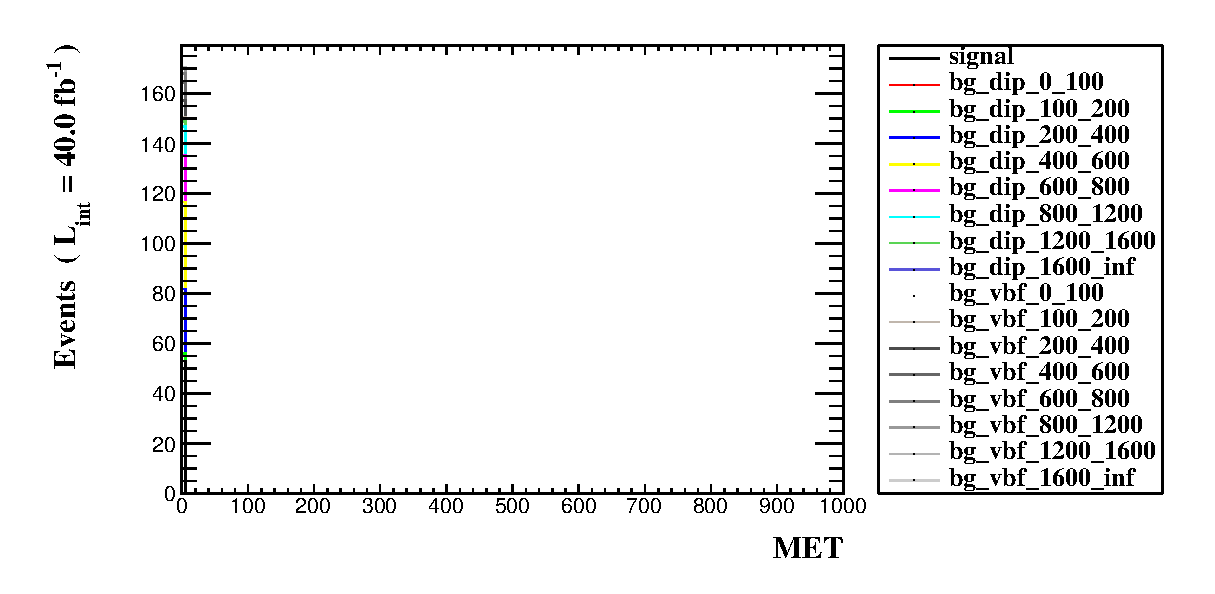
\includegraphics[scale=0.45]{selection_13.eps}\\
\caption{   }
  \end{center}
\end{figure}
      \newpage
\subsection{ Histogram 15}

\textbf{* Plot: TET}\\
   \begin{table}[H]
  \begin{center}
    \begin{tabular}{|m{23.0mm}|m{23.0mm}|m{18.0mm}|m{19.0mm}|m{19.0mm}|m{19.0mm}|m{19.0mm}|}
      \hline
      {\cellcolor{yellow}         Dataset}& {\cellcolor{yellow}         Integral}& {\cellcolor{yellow}         Entries per event}& {\cellcolor{yellow}         Mean}& {\cellcolor{yellow}         RMS}& {\cellcolor{yellow}         \% underflow}& {\cellcolor{yellow}         \% overflow}\\
      \hline
      {\cellcolor{white}         signal}& {\cellcolor{white}         52.9}& {\cellcolor{white}         1.0}& {\cellcolor{white}         1870.34}& {\cellcolor{white}         827.6}& {\cellcolor{green}         0.0}& {\cellcolor{green}         0.004039}\\
      \hline
      {\cellcolor{white}         bg\_dip\_0\_100}& {\cellcolor{white}         0.0 +/\-- 0.0}& {\cellcolor{white}         0.}& {\cellcolor{white}         0.0}& {\cellcolor{white}         0.0}& {\cellcolor{green}         0.0}& {\cellcolor{green}         0.0}\\
      \hline
      {\cellcolor{white}         bg\_dip\_100\_200}& {\cellcolor{white}         3.16}& {\cellcolor{white}         1.0}& {\cellcolor{white}         728.733}& {\cellcolor{white}         80.65}& {\cellcolor{green}         0.0}& {\cellcolor{green}         0.0}\\
      \hline
      {\cellcolor{white}         bg\_dip\_200\_400}& {\cellcolor{white}         25.8}& {\cellcolor{white}         1.0}& {\cellcolor{white}         914.659}& {\cellcolor{white}         167.9}& {\cellcolor{green}         0.0}& {\cellcolor{green}         0.0}\\
      \hline
      {\cellcolor{white}         bg\_dip\_400\_600}& {\cellcolor{white}         34.8}& {\cellcolor{white}         1.0}& {\cellcolor{white}         1085.81}& {\cellcolor{white}         190.6}& {\cellcolor{green}         0.0}& {\cellcolor{green}         0.0}\\
      \hline
      {\cellcolor{white}         bg\_dip\_600\_800}& {\cellcolor{white}         18.8}& {\cellcolor{white}         1.0}& {\cellcolor{white}         1355.7}& {\cellcolor{white}         222.6}& {\cellcolor{green}         0.0}& {\cellcolor{green}         0.0}\\
      \hline
      {\cellcolor{white}         bg\_dip\_800\_1200}& {\cellcolor{white}         11.4}& {\cellcolor{white}         1.0}& {\cellcolor{white}         1717.84}& {\cellcolor{white}         310.2}& {\cellcolor{green}         0.0}& {\cellcolor{green}         0.0}\\
      \hline
      {\cellcolor{white}         bg\_dip\_1200\_1600}& {\cellcolor{white}         1.92}& {\cellcolor{white}         1.0}& {\cellcolor{white}         2223.42}& {\cellcolor{white}         420.2}& {\cellcolor{green}         0.0}& {\cellcolor{green}         0.0}\\
      \hline
      {\cellcolor{white}         bg\_dip\_1600\_inf}& {\cellcolor{white}         0.492}& {\cellcolor{white}         1.0}& {\cellcolor{white}         2762.71}& {\cellcolor{white}         554.7}& {\cellcolor{green}         0.0}& {\cellcolor{green}         0.0}\\
      \hline
      {\cellcolor{white}         bg\_vbf\_0\_100}& {\cellcolor{white}         0.0486}& {\cellcolor{white}         1.0}& {\cellcolor{white}         814.434}& {\cellcolor{white}         141.3}& {\cellcolor{green}         0.0}& {\cellcolor{green}         0.0}\\
      \hline
      {\cellcolor{white}         bg\_vbf\_100\_200}& {\cellcolor{white}         1.16}& {\cellcolor{white}         1.0}& {\cellcolor{white}         822.463}& {\cellcolor{white}         164.7}& {\cellcolor{green}         0.0}& {\cellcolor{green}         0.0}\\
      \hline
      {\cellcolor{white}         bg\_vbf\_200\_400}& {\cellcolor{white}         6.68}& {\cellcolor{white}         1.0}& {\cellcolor{white}         911.682}& {\cellcolor{white}         196.9}& {\cellcolor{green}         0.0}& {\cellcolor{green}         0.0}\\
      \hline
      {\cellcolor{white}         bg\_vbf\_400\_600}& {\cellcolor{white}         7.09}& {\cellcolor{white}         1.0}& {\cellcolor{white}         1092.69}& {\cellcolor{white}         207.8}& {\cellcolor{green}         0.0}& {\cellcolor{green}         0.0}\\
      \hline
      {\cellcolor{white}         bg\_vbf\_600\_800}& {\cellcolor{white}         3.66}& {\cellcolor{white}         1.0}& {\cellcolor{white}         1358.1}& {\cellcolor{white}         214.6}& {\cellcolor{green}         0.0}& {\cellcolor{green}         0.0}\\
      \hline
      {\cellcolor{white}         bg\_vbf\_800\_1200}& {\cellcolor{white}         2.15}& {\cellcolor{white}         1.0}& {\cellcolor{white}         1733.69}& {\cellcolor{white}         293.4}& {\cellcolor{green}         0.0}& {\cellcolor{green}         0.0}\\
      \hline
      {\cellcolor{white}         bg\_vbf\_1200\_1600}& {\cellcolor{white}         0.385}& {\cellcolor{white}         1.0}& {\cellcolor{white}         2285.17}& {\cellcolor{white}         379.1}& {\cellcolor{green}         0.0}& {\cellcolor{green}         0.0}\\
      \hline
      {\cellcolor{white}         bg\_vbf\_1600\_inf}& {\cellcolor{white}         0.0982}& {\cellcolor{white}         1.0}& {\cellcolor{white}         2919.31}& {\cellcolor{white}         576.8}& {\cellcolor{green}         0.0}& {\cellcolor{green}         0.0}\\
\hline
    \end{tabular}
  \end{center}
\end{table}

\begin{figure}[H]
  \begin{center}
    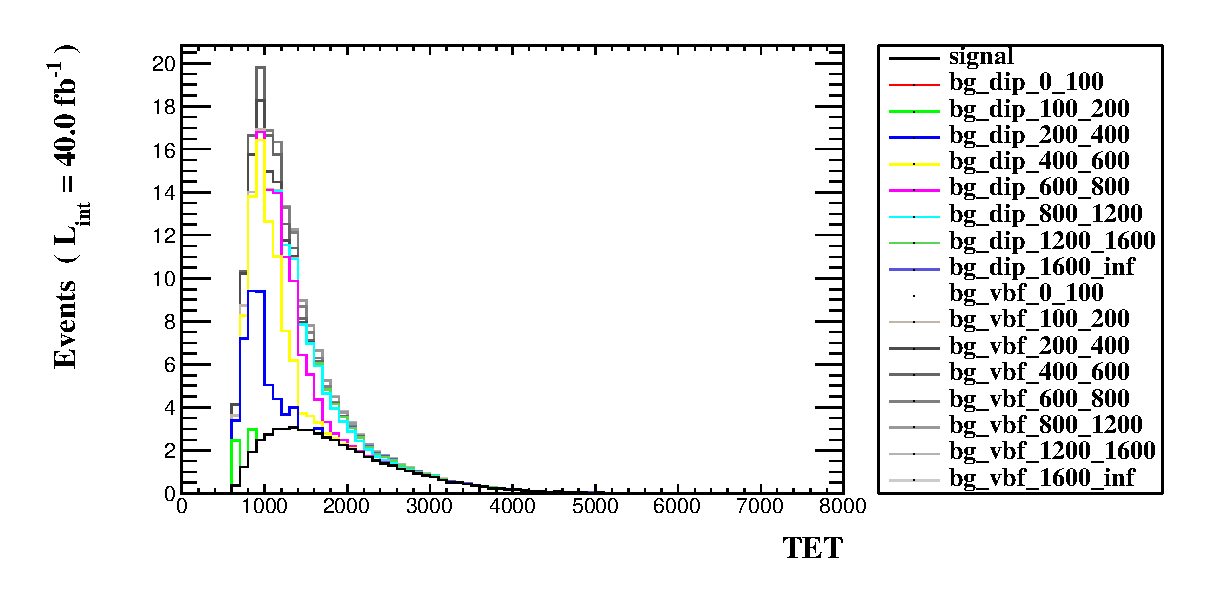
\includegraphics[scale=0.45]{selection_14.eps}\\
\caption{   }
  \end{center}
\end{figure}
      % -----------------------------------------------------------------------------
%                                SECTION Summary                                
% -----------------------------------------------------------------------------
\newpage
\section{ Summary}

\subsection{Cut-flow charts}

\begin{itemize}
  \item How to compare signal (S) and background (B): \textcolor{blue}{S/\-sqrt(S+B+(xB)**2)} .
   \item Object definition selections are indicated in cyan.  \item Reject and select are indicated by 'REJ' and 'SEL' respectively
\end{itemize}
\begin{table}[H]
  \begin{center}
    \begin{tabular}{|m{36.0mm}|m{36.0mm}|m{36.0mm}|m{33.0mm}|}
      \hline
      {\cellcolor{yellow}        Cuts}& {\cellcolor{yellow}         Signal (S)}& {\cellcolor{yellow}         Background (B)}& {\cellcolor{yellow}         S vs B}\\
      \hline
      {\cellcolor{white}         Initial (no cut)}& {\cellcolor{white}         106.858 +/\-- 0.148}& {\cellcolor{white}         4113516 +/\-- 4877}& {\cellcolor{white}         1.04e-04 +/\-- 9.46e-08}\\
      \hline
      {\cellcolor{white} SEL: ( ( sdETA ( jets[1] jets[2] ) > 2.0 or sdETA }& {\cellcolor{white}         52.67 +/\-- 5.17}& {\cellcolor{white}         117.7 +/\-- 10.8}& {\cellcolor{white}         1.636 +/\-- 0.115}\\
\hline
    \end{tabular}
  \end{center}
\end{table}

\end{document}
